\section{Praktische Anwendung der FM-Synthese}
\FloatBarrier
\subsection{Nachbildung eines Instrumentes}
Da es bei der FM-Synthese schwer fällt vorauszusagen, wie das durch die Synthese erzeugte Spektrum aussehen wird, ist es ein schwieriges Unterfangen mit dieser Technik ein echt wirkendes Instrument nachzubilden, siehe \ref{PrinzipFM} - \nameref{PrinzipFM}.
Trotzdem gibt es einige Techniken den generierten Klang natürlicher wirken zu lassen. Diese werden im weiteren Verlauf dieses Kapitels vorgestellt und anschließend wird der Versuch unternommen das Klangbild eines Querflötentones nachzubilden.

\FloatBarrier
\subsubsection{Techniken zur Nachbildung eines Instrumententones mittels FM-Synthese}

Bei der Synthese eines Tones mittels FM-Synthese müssen zunächst die Parameter der FM-Synthese Formel festgelegt werden. Hierzu kann das Frequenzspektrum und das Spektrogramm des nachzubildenden Tones verwendet werden. Eine ausführliche Erklärung der einzelnen Parameter ist zu finden in Kapitel \ref{einfacheFM} - \nameref{einfacheFM}. 

Mit dem Offensichtlichstem kann gestartet werden, der Grundfrequenz. Sie ist die niedrigste ausgeprägte Frequenz des Spektrums und legt die Tonhöhe fest \cite[S. 53]{barkowsky}. Sie kann als Trägerfrequenz $f_c$ verwendet werden. Der Abstand der einzelnen Frequenzen zueinander ist der zweite Anhaltspunkt. Dieser Abstand findet als Modulationsfrequenz $f_m$ Verwendung. Für harmonische Töne ist ein ganzzahliges Vielfaches der Grundfrequenz als Modulationsfrequenz nötig \cite[S. 528]{chowningPaper}. Der Modulationsindex $I$ kann mithilfe der Bessel Funktionen gefunden werden - siehe hierzu \ref{bulli:besselModIndexZusammenahang} - \nameref{bulli:besselModIndexZusammenahang}. Alternativ kann eine grobe Schätzung vorgenommen werden, hierzu ist die folgende Faustformel nützlich:

\begin{equation}
\label{eq:faustformel}
I + 1 = \text{Anzahl der Seitenfrequenzen mit signifikanter Ausprägung}
\end{equation}

Die Formel in \ref{eq:faustformel} kann mit Hilfe der Formel der Bandbreite aus \ref{eq:fmBandwidth} hergeleitet werden \cite[S. 221]{lathi}. Sollte mittels der normalen FM-Synthese kein zufriedenstellendes Ergebnis erzielt werden können, kann mit der komplexen FM-Synthese experimentiert werden. 

Bei der komplexen FM-Synthese finden mehrere Träger oder mehrere Modulatoren Verwendung. Diese können in Reihe oder parallel geschaltet werden. Außerdem kann auch die so genannte Feedback Frequenzmodulation genutzt werden, welche das Signal mit dem jeweils voran gegangenem Sample moduliert \cite[S. 399 f.]{hornerPaper}. Feedback-FM-Synthese kann außerdem eingesetzt werden um Rauschen zu erzeugen. Sie kann aber auch ein sehr komplexes Spektrum mit besonders vielen Seitenfrequenzen erzeugen. Die komplexe FM-Synthese findet Einsatz, wenn mit der normalen FM-Synthese nicht ausreichend komplexe Spektren erzeugt werden können. Dies kann zum Beispiel der Fall sein, wenn mehrere exponentiell fallende Seitenfrequenzen erzeugt werden sollen. Wenn bei einfacher FM-Synthese der Modulationsindex erhöht wird um mehr Seitenfrequenzen zu erzeugen, verändert sich die Stärke der Grundfrequenz, definiert durch die Bessel Funktionen - nachzulesen im Kapitel \ref{bulli:besselModIndexZusammenahang} - \nameref{bulli:besselModIndexZusammenahang}. Um dies zu vermeiden muss auf die komplexe FM-Synthese zurückgegriffen werden, siehe \ref{PrinzipKomplexFM} - \nameref{PrinzipKomplexFM}

Eines der wichtigsten Grundbestandteile eines jeden Instrumententones ist die so genannte ADSR-Hüllkurve. Die Hüllkurve wird genutzt um die Amplitude des künstlich erzeugten Signals über den zeitlichen Verlauf festzulegen \cite[S. 532f]{chowningPaper}. ADSR steht für die einzelnen Phasen eines Tones: Attack, Decay, Sustain und Release. Diese Phasen sollen hier vereinfacht erklärt werden. Beim Drücken einer Taste wird der Ton angeschlagen und die Lautstärke des Tones steigt schnell bis zu einem maximalen Wert an. Diese Phase wird Attack genannt. Nachdem die maximale Lautstärke erreicht wurde, startet die Decay Phase. In dieser Phase sinkt die Lautstärke schnell auf einen geringeren Wert ab. Danach befindet sich der Ton, solange die Taste gedrückt wird, in der Sustain Phase und die Lautstärke bleibt konstant oder fällt leicht ab. Sobald die Taste losgelassen wird, befindet sich der Ton in der Release Phase und die Lautstärke nimmt wieder bis zu ihrem minimal Wert ab. In Abbildung \ref{fig:adsrDefault} ist der Verlauf der Lautstärke einer Standard ADSR-Hüllkurve noch einmal grafisch dargestellt.

\begin{figure} [ht]
\centering
  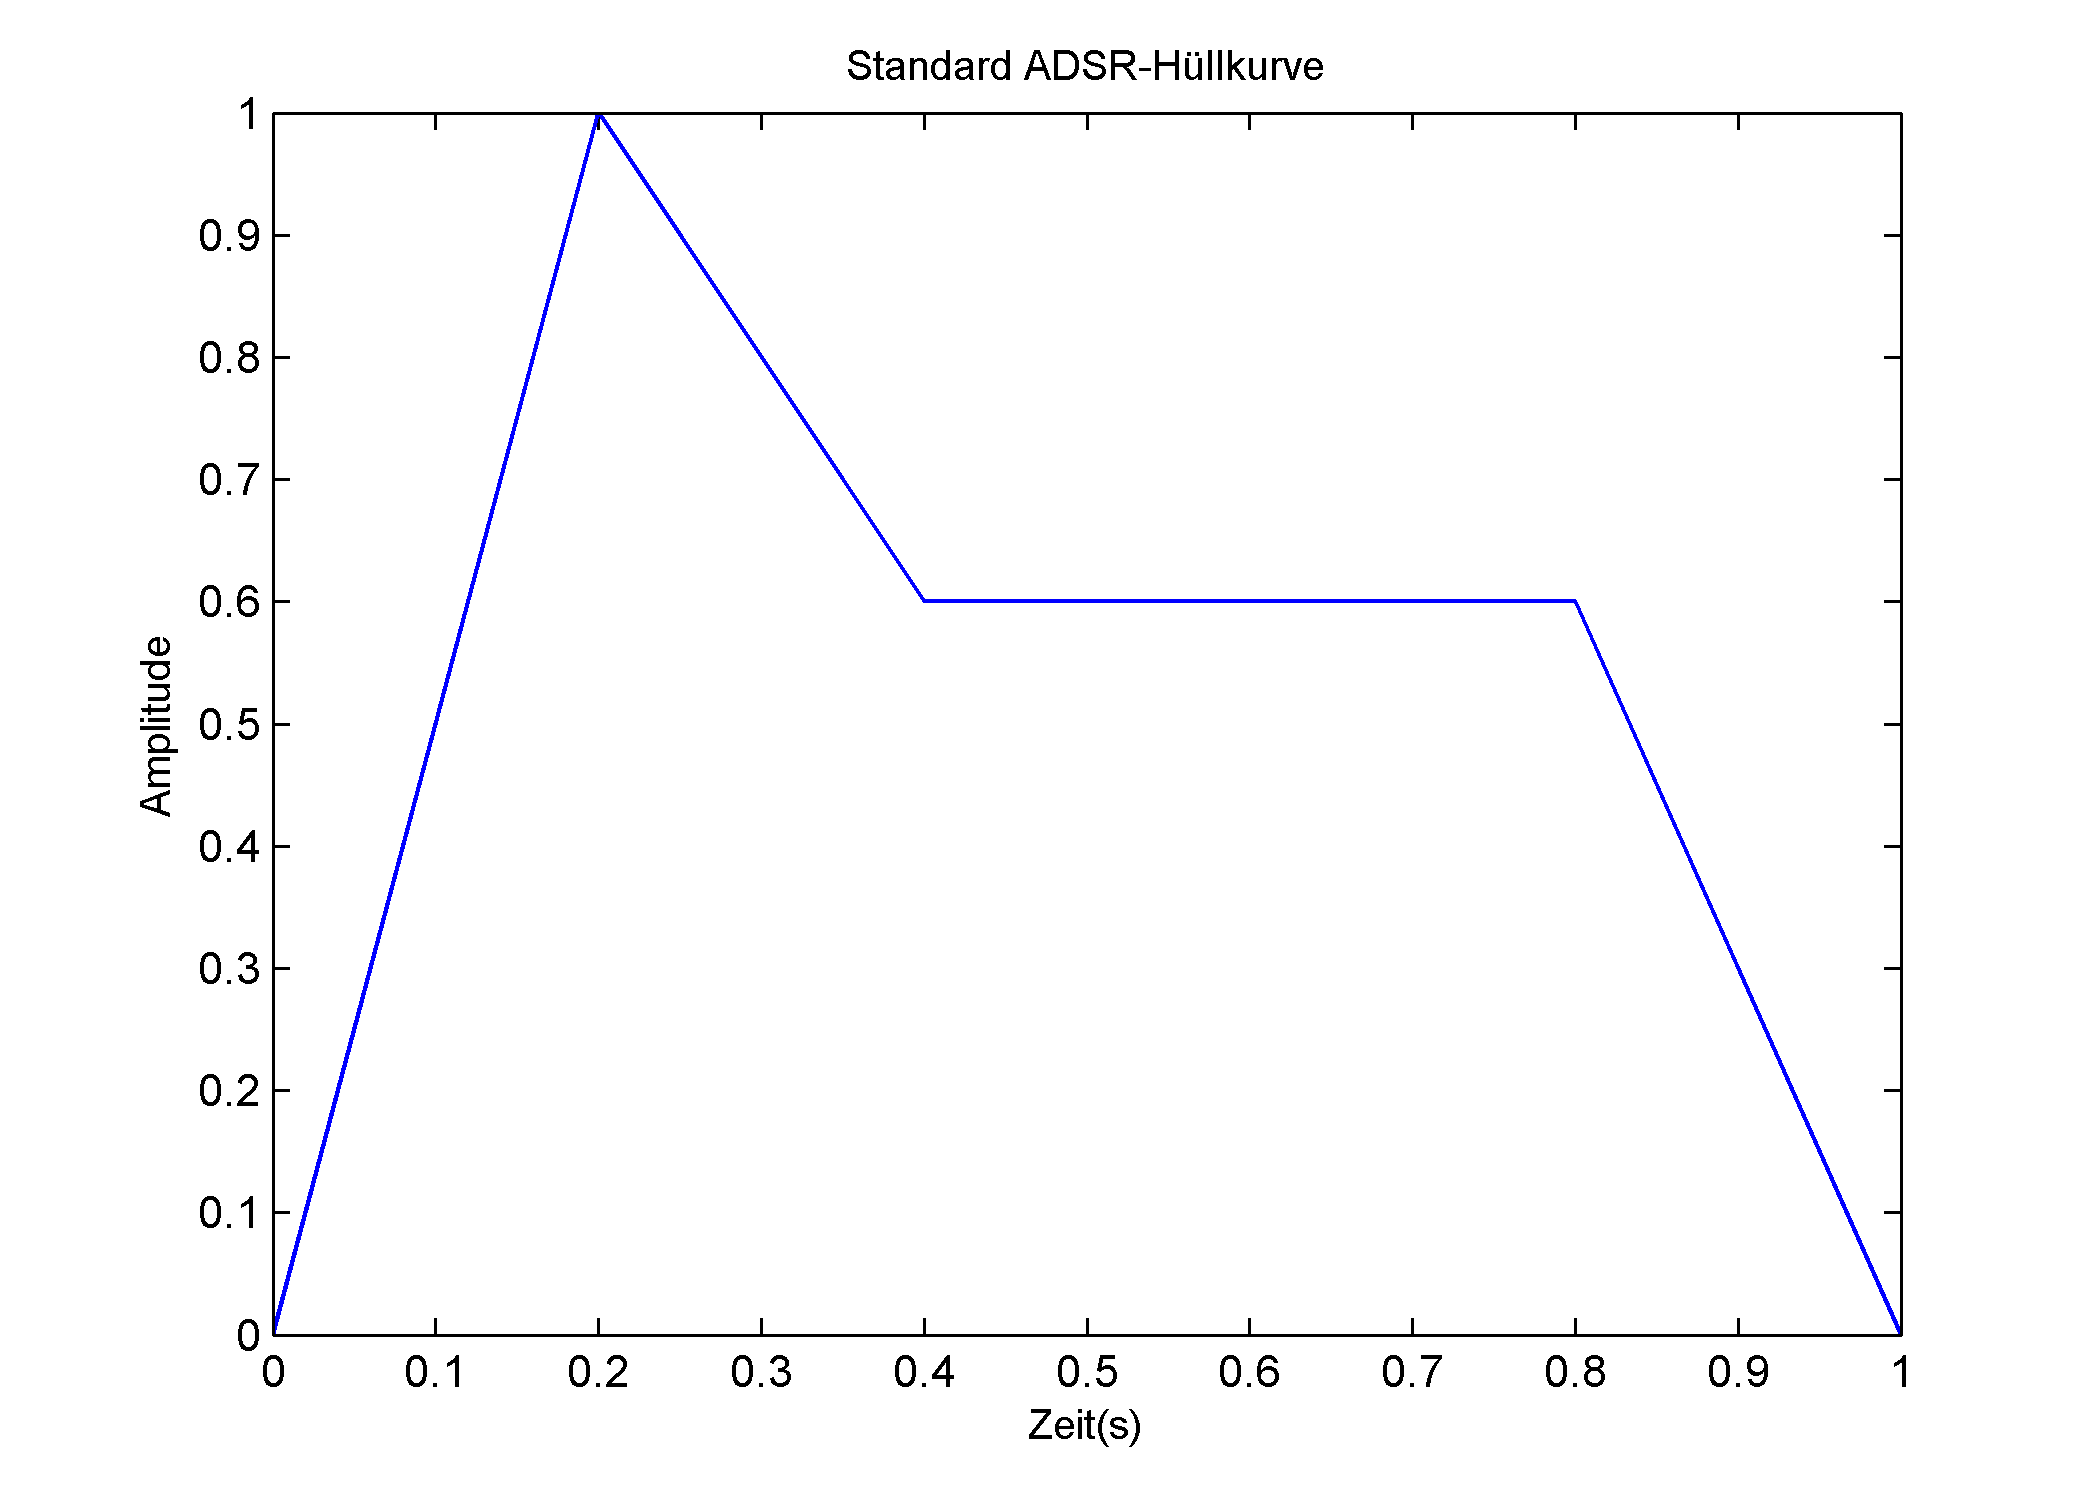
\includegraphics[width=0.5\textwidth]{adsrDefault.png}
\caption{Standard ADSR-Hüllkurve}
\label{fig:adsrDefault}
\end{figure}

Da allerdings bei vielen Instrumenten die Lautstärke in den einzelnen Phasen der ADSR-Hüllkurve nicht gleichmäßig steigt oder sinkt, ist es nötig beliebig komplexe Kurven abbilden zu können. Bei vielen Instrumenten steigt beispielsweise die Lautstärke in der Attack Phase exponentiell an und fällt in der Decay und Release Phase auch wieder exponentiell ab. Manche Synthesizer bieten zusätzlich auch noch eine Hold Phase vor der Attack Phase, für Instrumente, die einige Zeit benötigen, bis sie nach dem Anschlagen des Tones in die Attack Phase eintreten. In Abbildung \ref{fig:adsrTypical} wurden weitere für Instrumenten typische Hüllkurven dargestellt um zu verdeutlichen, dass die ADSR-Hüllkurve bei Instrumenten beliebig schlichte sowie komplexe Formen annehmen kann.

\begin{figure} [ht]
\centering
  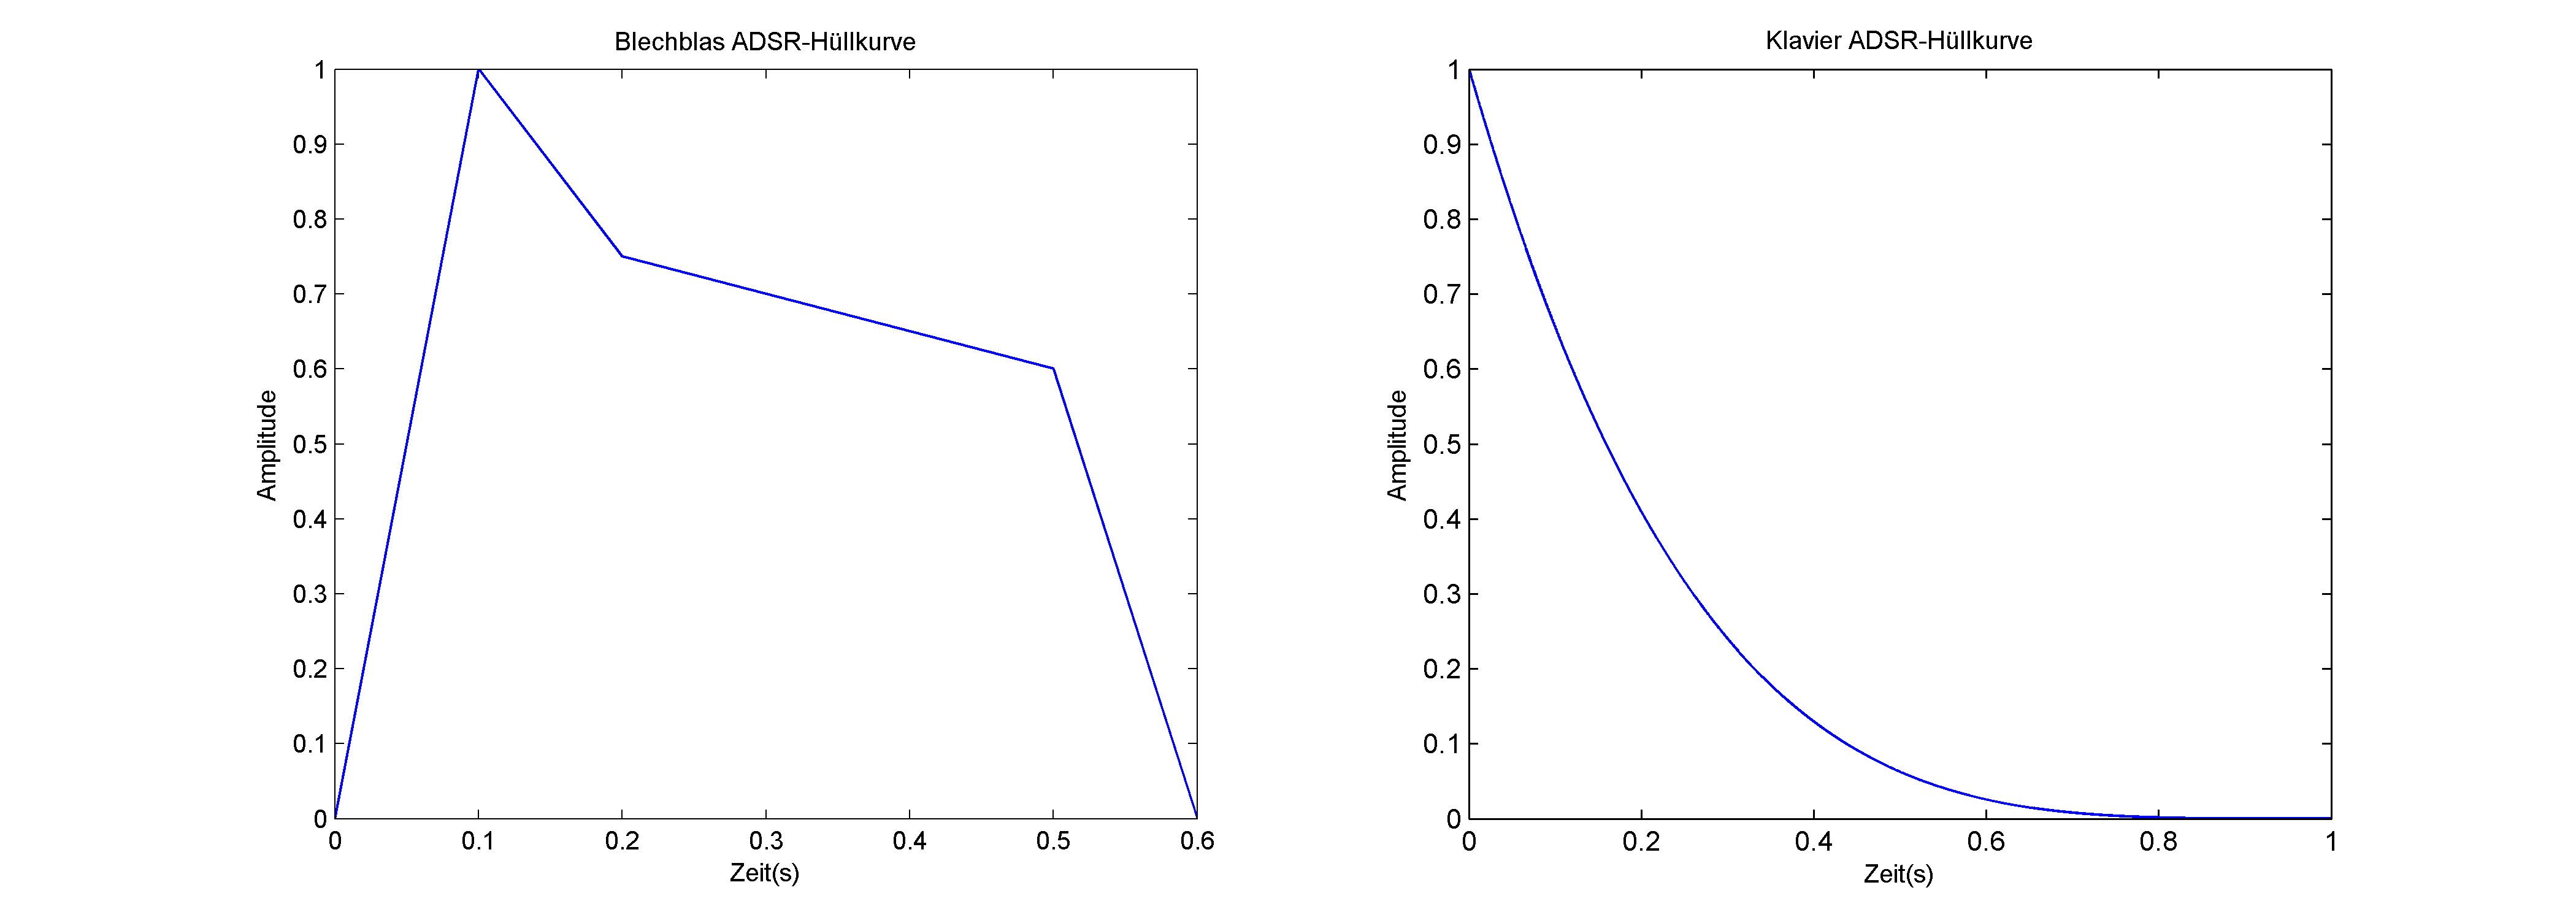
\includegraphics[width=1\textwidth]{adsrTypical.png}
\caption{Typische ADSR-Hüllkurve eines Blechblasinstrumentes \cite{chowningPaper} und eines Klaviers}
\label{fig:adsrTypical} 
\end{figure}

Auch wenn das Hinzufügen einer ADSR-Hüllkurve den Klang des synthetisierten Tones schon natürlicher wirken lässt, hört sich der erzeugte Ton noch nicht wie ein echtes Instrument an. Eine weitere Möglichkeit ihn zu verbessern, stellt die Variierung des Modulationsindex über die Zeit oder die Amplitude dar. Somit kann die Anzahl der Seitenfrequenzen verändert werden, was zu einem lebendigeren Klang führt. \cite[S. 532]{chowningPaper}

Um den Klang des Tones noch weiter zu verbessern stellen Filter ein gutes Hilfsmittel dar. Filter können genutzt werden um das von der FM Synthese erzeugte Signal zu manipulieren. Dabei werden ungewollte Frequenzen gedämpft bzw. komplett herausgefiltert oder gewollte Frequenzen verstärkt. Typische Vertreter von Filtern sind Hochpassfilter, Tiefpassfilter, Bandpass und Bandsperre. \cite[S. 100-104]{stotz}

Das bisher erzeugte Signal ist noch ein reines Signal, welches so in der Natur nicht vorkommen kann. Bei Luftverwirbelungen und Unebenheiten des Instrumentes tritt Rauschen auf. Dieses Rauschen trägt zum typischen Klangbild eines Instrumentes bei und muss auch nachgebildet werden. Ein Rauschen kann mittels Feedback-FM-Synthese erzeugt werden, dafür muss der Modulationsindex sehr hoch angesetzt werden. Das von der Feedback-FM-Synthese erzeugte Signal gleicht einem weißen Rauschen. Anschließend kann dieses Rauschen mittels Multibandpassfilter um die jeweiligen ausgeprägten Frequenzen gefiltert werden. Würde das Rauschen nicht gefiltert, kann neben dem Ton, das Rauschen als solches wahrgenommen werden. \cite[S. 152]{barkowsky}

Um den Klang des synthetisierten Tones noch natürlicher zu gestalten, könnte dem Ton zusätzlich ein Hall-Effekt hinzugefügt werden. Hall entsteht bei der diffusen Reflexion des Schalls an den Wänden eines Raumes, welche zu einer großen Anzahl an Echos führen. \cite[S. 108]{stotz}


\FloatBarrier
\subsubsection{Nachbildung des Klangbildes eines Querflötentones mittels FM-Synthese}

Im Laufe dieses Kapitels soll ein Ton einer Querflöte mittels FM-Synthese erzeugt und mit den oben beschriebenen Techniken verfeinert werden. Das Instrument Querflöte wurde ausgewählt, da es sehr harmonische Spektren erzeugt. Auf das nutzen eines Instrumentes mit einem inharmonischen Spektrum wurde vorsätzlich verzichtet, da die FM-Synthese mit harmonischen Spektren kontrollierbarer ist. Alle Beispiele sind in Matlab erstellt und können mit den beiliegenden Source-Code nachgestellt werden. In Abbildung \ref{fig:plotFluteOrig} sind Spektrogramm, Waveform und Spektrum des originalen Querflötentones abgebildet. Mit den Informationen aus den vorliegenden Grafiken wird versucht, dieses spezifische Klangbild nachzubilden.

\begin{figure} [h!t!b!]
\centering
  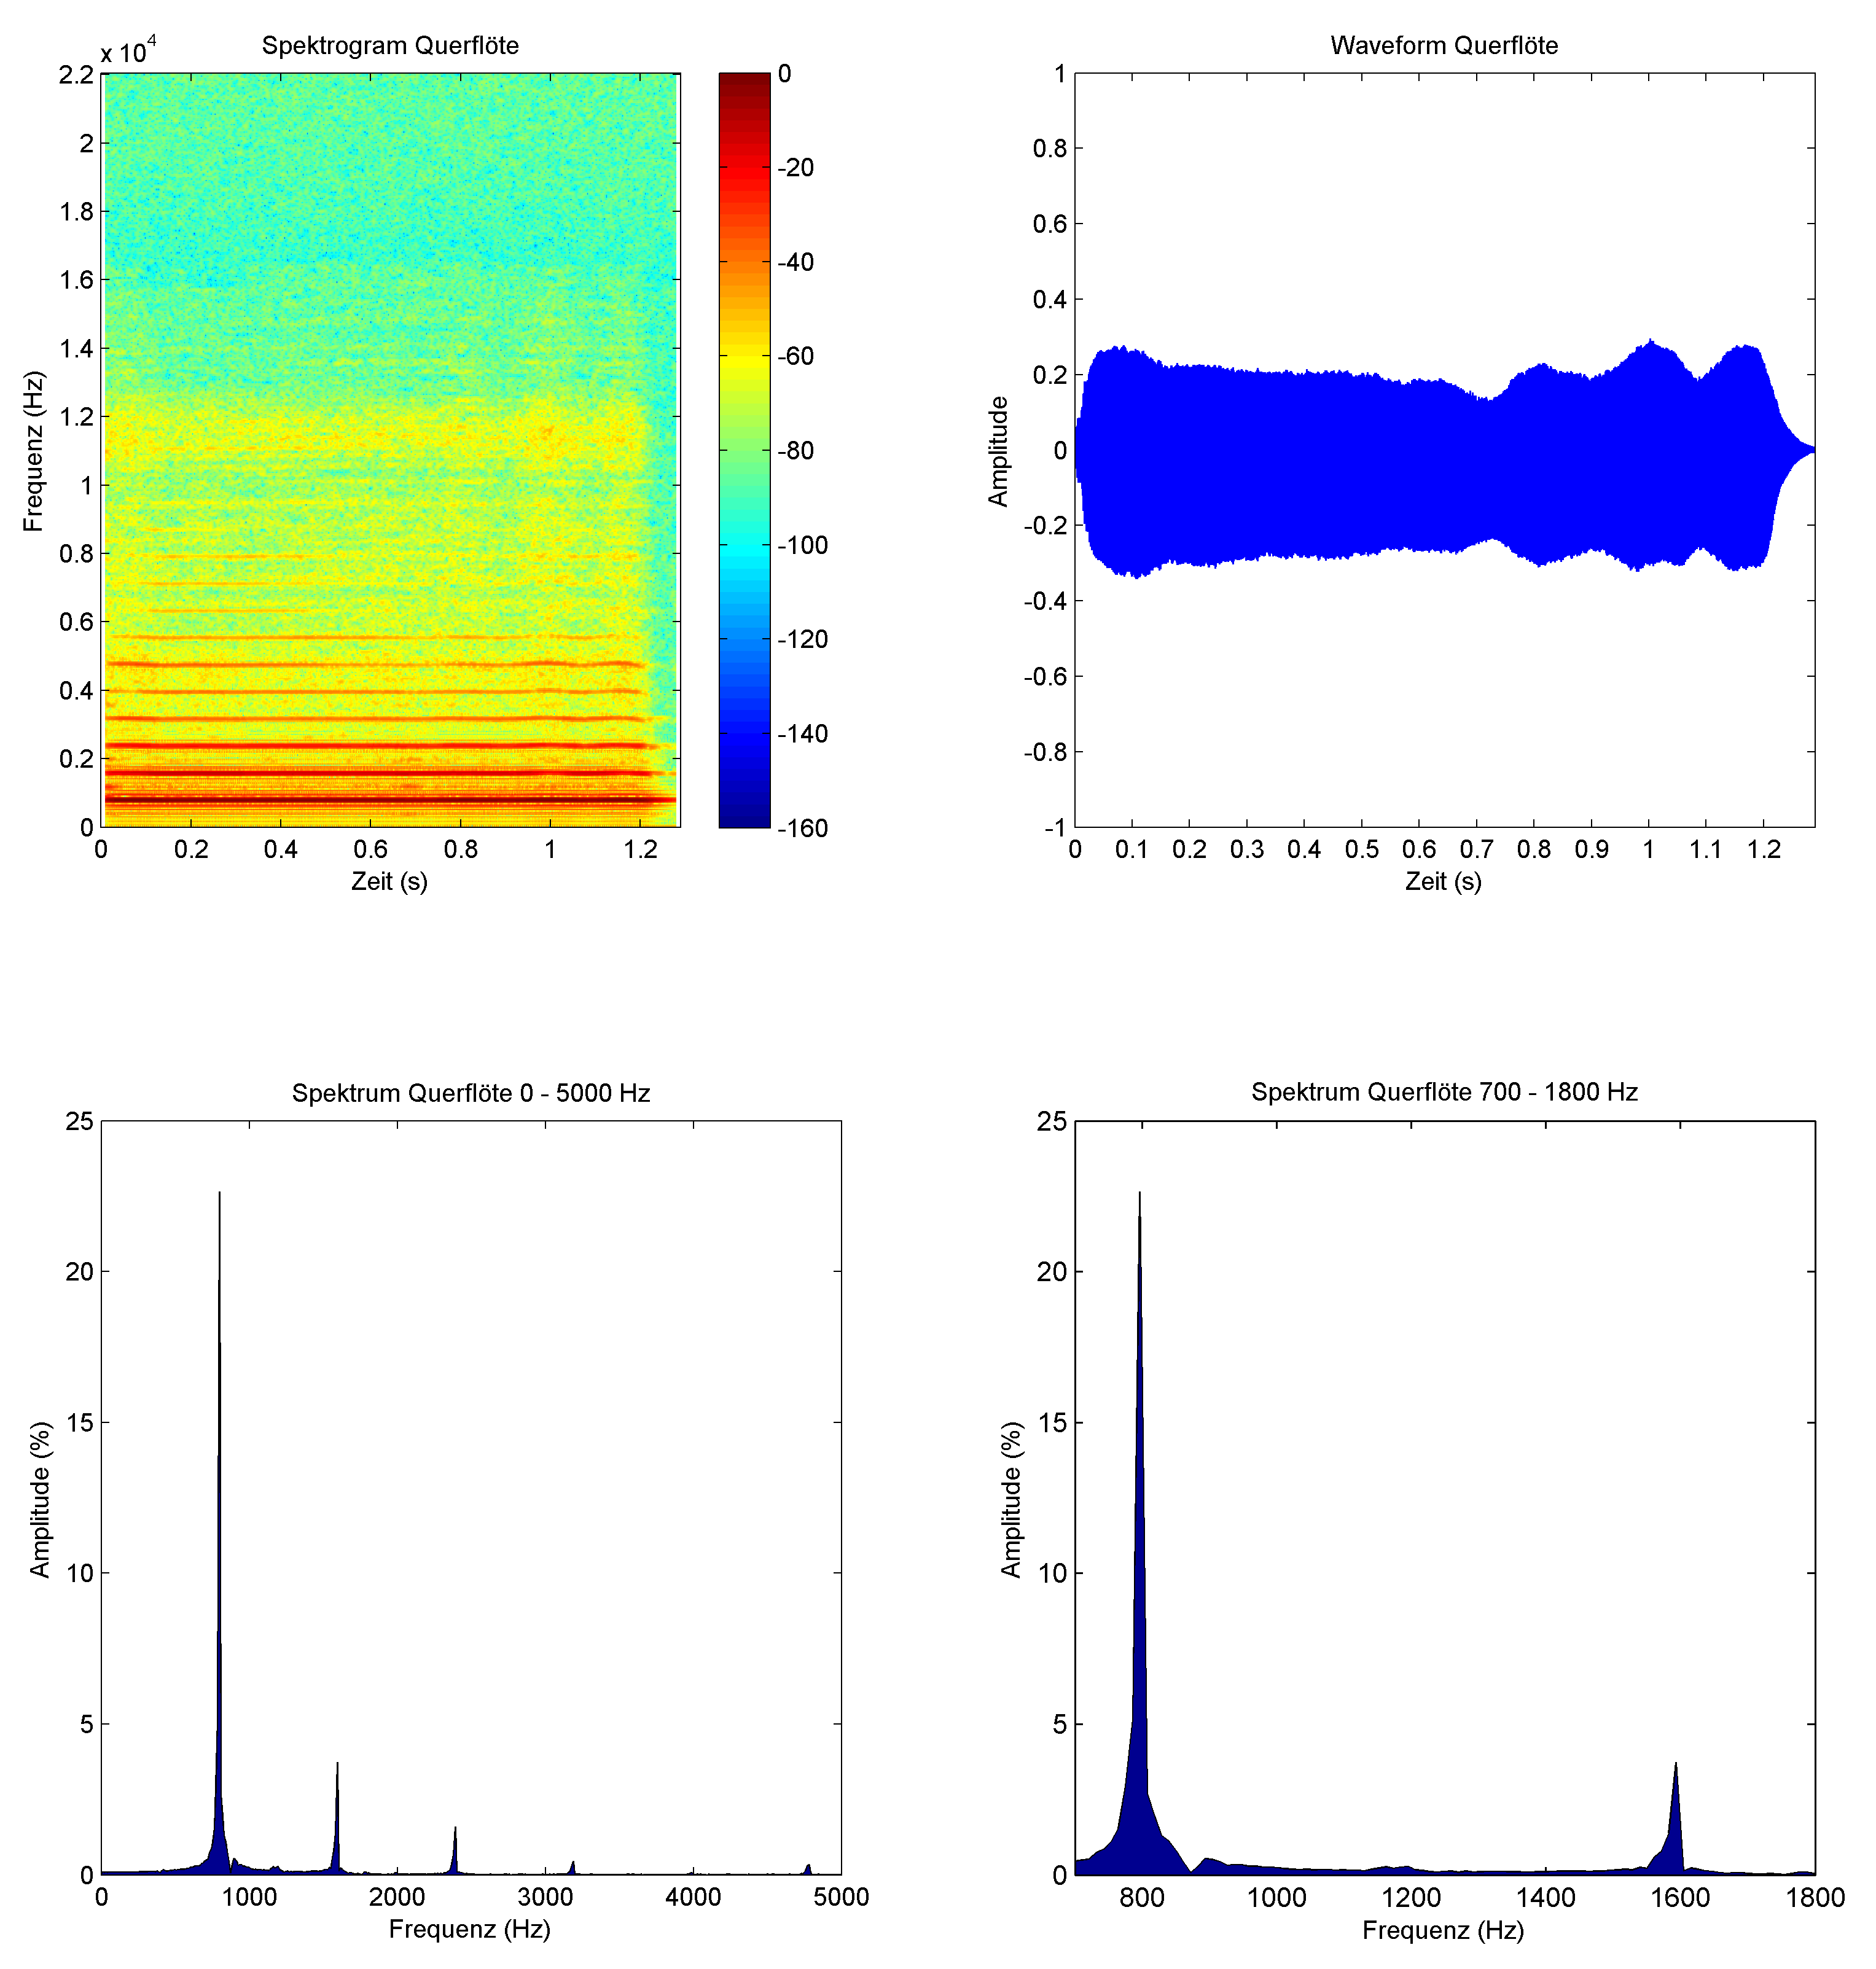
\includegraphics[width=1\textwidth]{plotFluteOrig.png}
\caption{Plot des Spektrogramms, der Waveform und des Spektrums eines echten Tones einer Querflöte}
\label{fig:plotFluteOrig}
\end{figure}

Anhand des Spektrums können bereits einige Erkenntnisse für die FM-Synthese gewonnen werden. Zunächst ist zu bemerken, dass die Grundfrequenz am stärksten ausgeprägt ist und bei etwa 800 Hz liegt. Um das Klangbild möglichst genau nachzubilden, muss die Frequenz allerdings durch vergrößern der Grafik ausgelesen werden. Bei dieser genaueren Betrachtung wird sichtbar, dass die Frequenz bei 791 Hz ihren maximalen Ausschlag erreicht. Diese Frequenz wird bei der FM-Synthese als Trägerfrequenz $f_c$ genutzt. Der Klang entspricht somit am ehesten einem G5 (in deutscher Notation einem g\textsuperscript{2}) mit 784 Hz \cite[S. 181]{borucki}. Im Spektrum sind außerdem noch mehrere Seitenfrequenzen zu erkennen. Die erste dieser Seitenfrequenzen befindet sich bei etwa dem doppelten der Grundfrequenz. Bei erneuter genauerer Betrachtung wird erkennbar, dass sie ihren maximalen Amplitudenwert bei exakt dem doppeltem der Grundfrequenz (1582 Hz) hat. Somit ist der Abstand zwischen Grundfrequenz und erster Seitenfrequenz genauso groß wie die Grundfrequenz selbst. Hierbei ist zu bemerken, dass der Abstand von einem ganzzahligen Multiplikator mit der Grundfrequenz typisch für einen harmonischen Klang ist \cite[S. 528]{chowningPaper}. Die nächsten Seitenfrequenzen haben jeweils wieder denselben Abstand von 791 Hz zur jeweiligen vorangegangenen Seitenfrequenz. Aus dieser Beobachtung kann die Modulationsfrequenz $f_m$ von 791 Hz geschlossen werden. Anhand der Anzahl der sichtbaren Seitenfrequenzen im Spektrum kann eine ungefähre Abschätzung des Modulationsindexes $I$ mit der Faustformel aus \ref{eq:faustformel} gewagt werden. Somit wird der Modulationsindex $I$ für die ersten Tests auf 0.5 eingestellt. 

\begin{figure} [ht]
\centering
  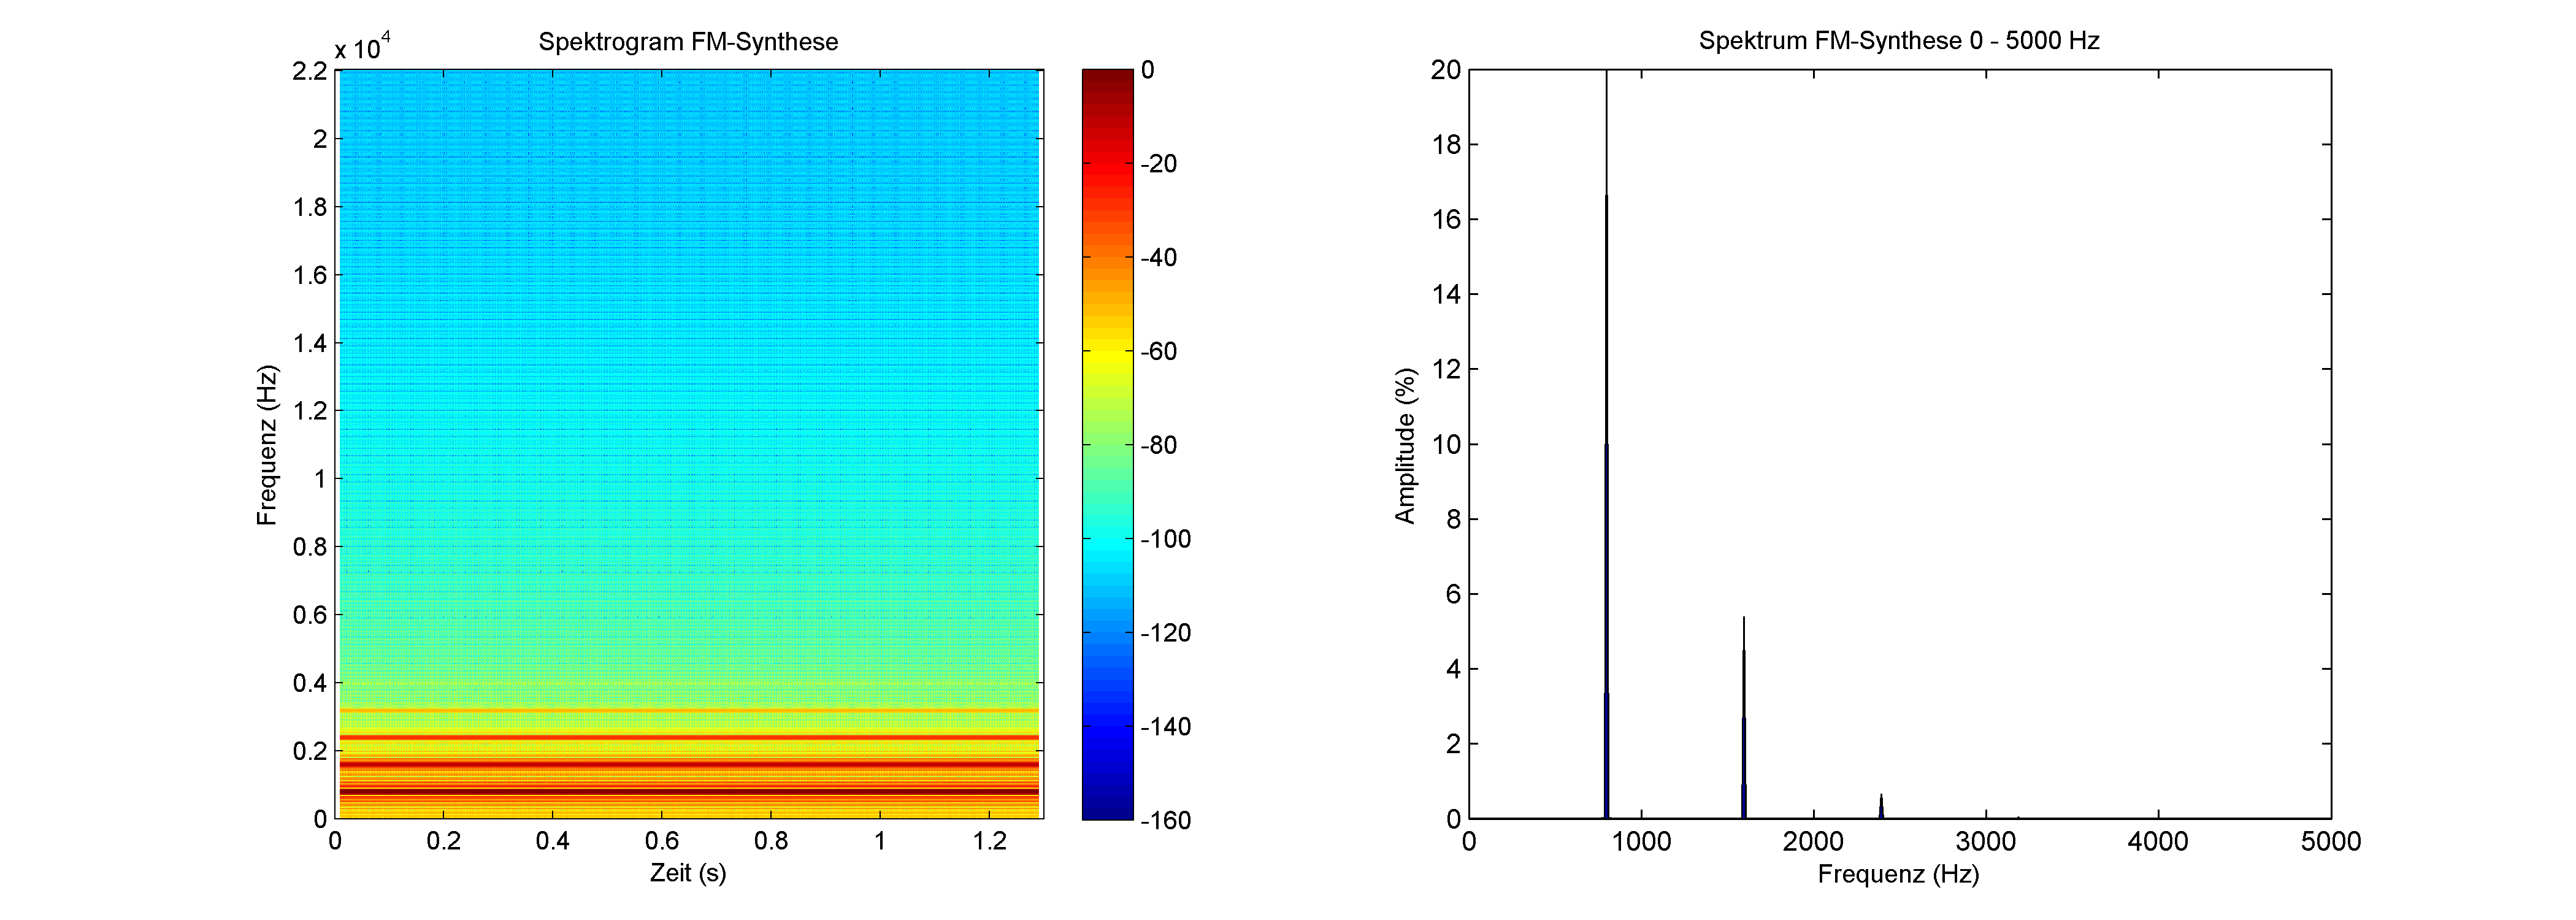
\includegraphics[width=1\textwidth]{plotFMSyntheseI05.png}
\caption{Plot des Spektrogramms und des Spektrums der FM-Synthese mit den Parametern $f_c = 791$ Hz, $f_m = f_c$ und $I = 0.5$ }
\label{fig:plotFMSyntheseI05}
\end{figure}

Ein erstes Spektrum der FM-Synthese mit den eben festgelegten Werten kann in Abbildung \ref{fig:plotFMSyntheseI05} begutachtet werden. Beim Evaluieren der Ergebnisse dieses Spektrums fällt auf, dass die erste Seitenfrequenz im Verhältnis zur Grundfrequenz einen viel stärkeren Ausschlag aufweist als es bei der Querflöte der Fall ist. Zudem fällt danach die Amplitude der 2. und 3. Seitenfrequenz viel stärker ab als bei dem Instrument. Untersucht man jetzt noch das Spektrogramm (ebenfalls in Abbildung \ref{fig:plotFMSyntheseI05}), fällt im Vergleich zum Spektrogramm der Querflöte die sehr viel geringere Anzahl an Seitenfrequenzen auf. Die Seitenfrequenzen bei 4000 Hz und darüber sind bei dem Instrument noch deutlich sichtbar während sie bei der FM-Synthese schon bei 4000 Hz kaum noch existent sind. Wird versucht den Modulationsindex zu erhöhen um die Anzahl der Seitenfrequenzen zu steigern, verlagert sich die Amplitude der Trägerfrequenz auf die Seitenfrequenzen, damit werden die Seitenfrequenzen stärker und die Trägerfrequenz schwächer, dargestellt in Abbildung \ref{fig:spektrumFMSyntheseI2}. 

\begin{figure} [ht]
\centering
  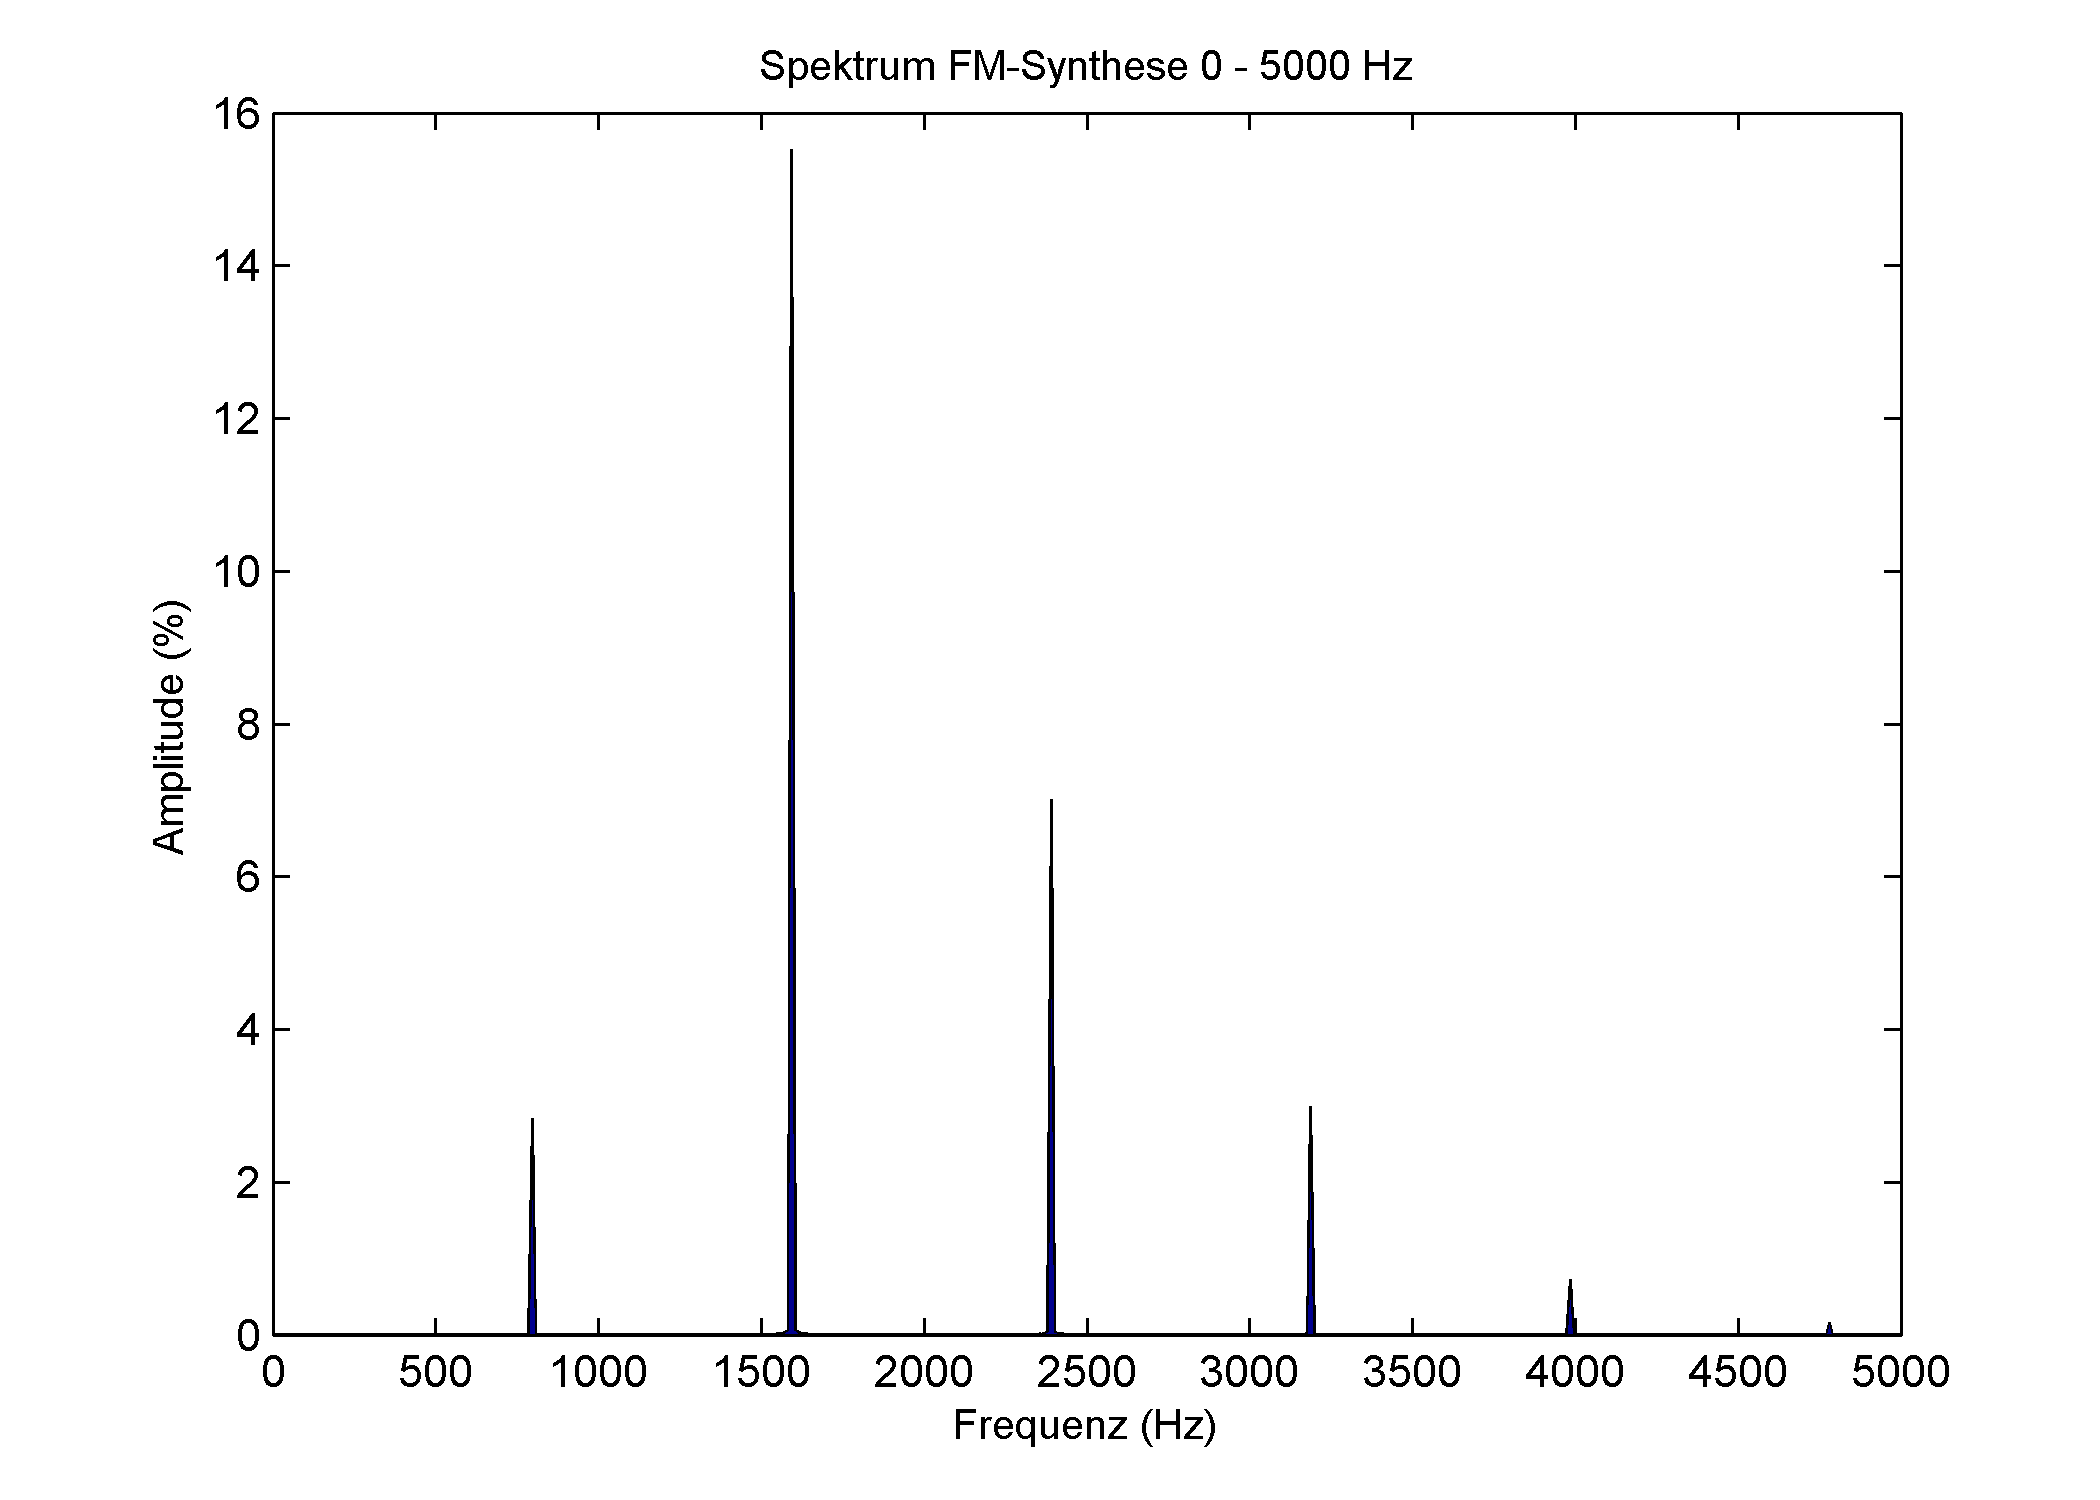
\includegraphics[width=0.5\textwidth]{spektrumFMSyntheseI2.png}
\caption{Plot des Spektrums der FM-Synthese mit den Parametern $f_c = 791 Hz$, $f_m = f_c$ und $I = 2$}
\label{fig:spektrumFMSyntheseI2}
\end{figure}

Um dieses Verhalten zu umgehen muss sich der komplexen FM-Synthese gewidment werden. Hierbei werden mehrere Modulatoren verschachtelt um eine größere Anzahl an Seitenfrequenzen zu erzeugen. Allerdings ist es bei der komplexen FM-Synthese, im Vergleich zur einfachen FM-Synthese, nochmal schwerer abzuschätzen wie stark die Amplituden der einzelnen Seitenfrequenzen ausgeprägt sein werden. Deshalb braucht es einige Experimente um auf das gewünschte Ergebnis zu stoßen. In Abbildung \ref{fig:plotFMSyntheseKomplex4Mod} kann das Resultat der FM-Synthese mit 4 Modulatoren betrachtet werden. Dieses Spektrum ähnelt dem der Querflöte schon sehr viel stärker und auch das Spektrogramm weißt in den Intensitäten der Seitenfrequenzen eine deutliche Ähnlichkeit auf.

\begin{figure} [ht]
\centering
  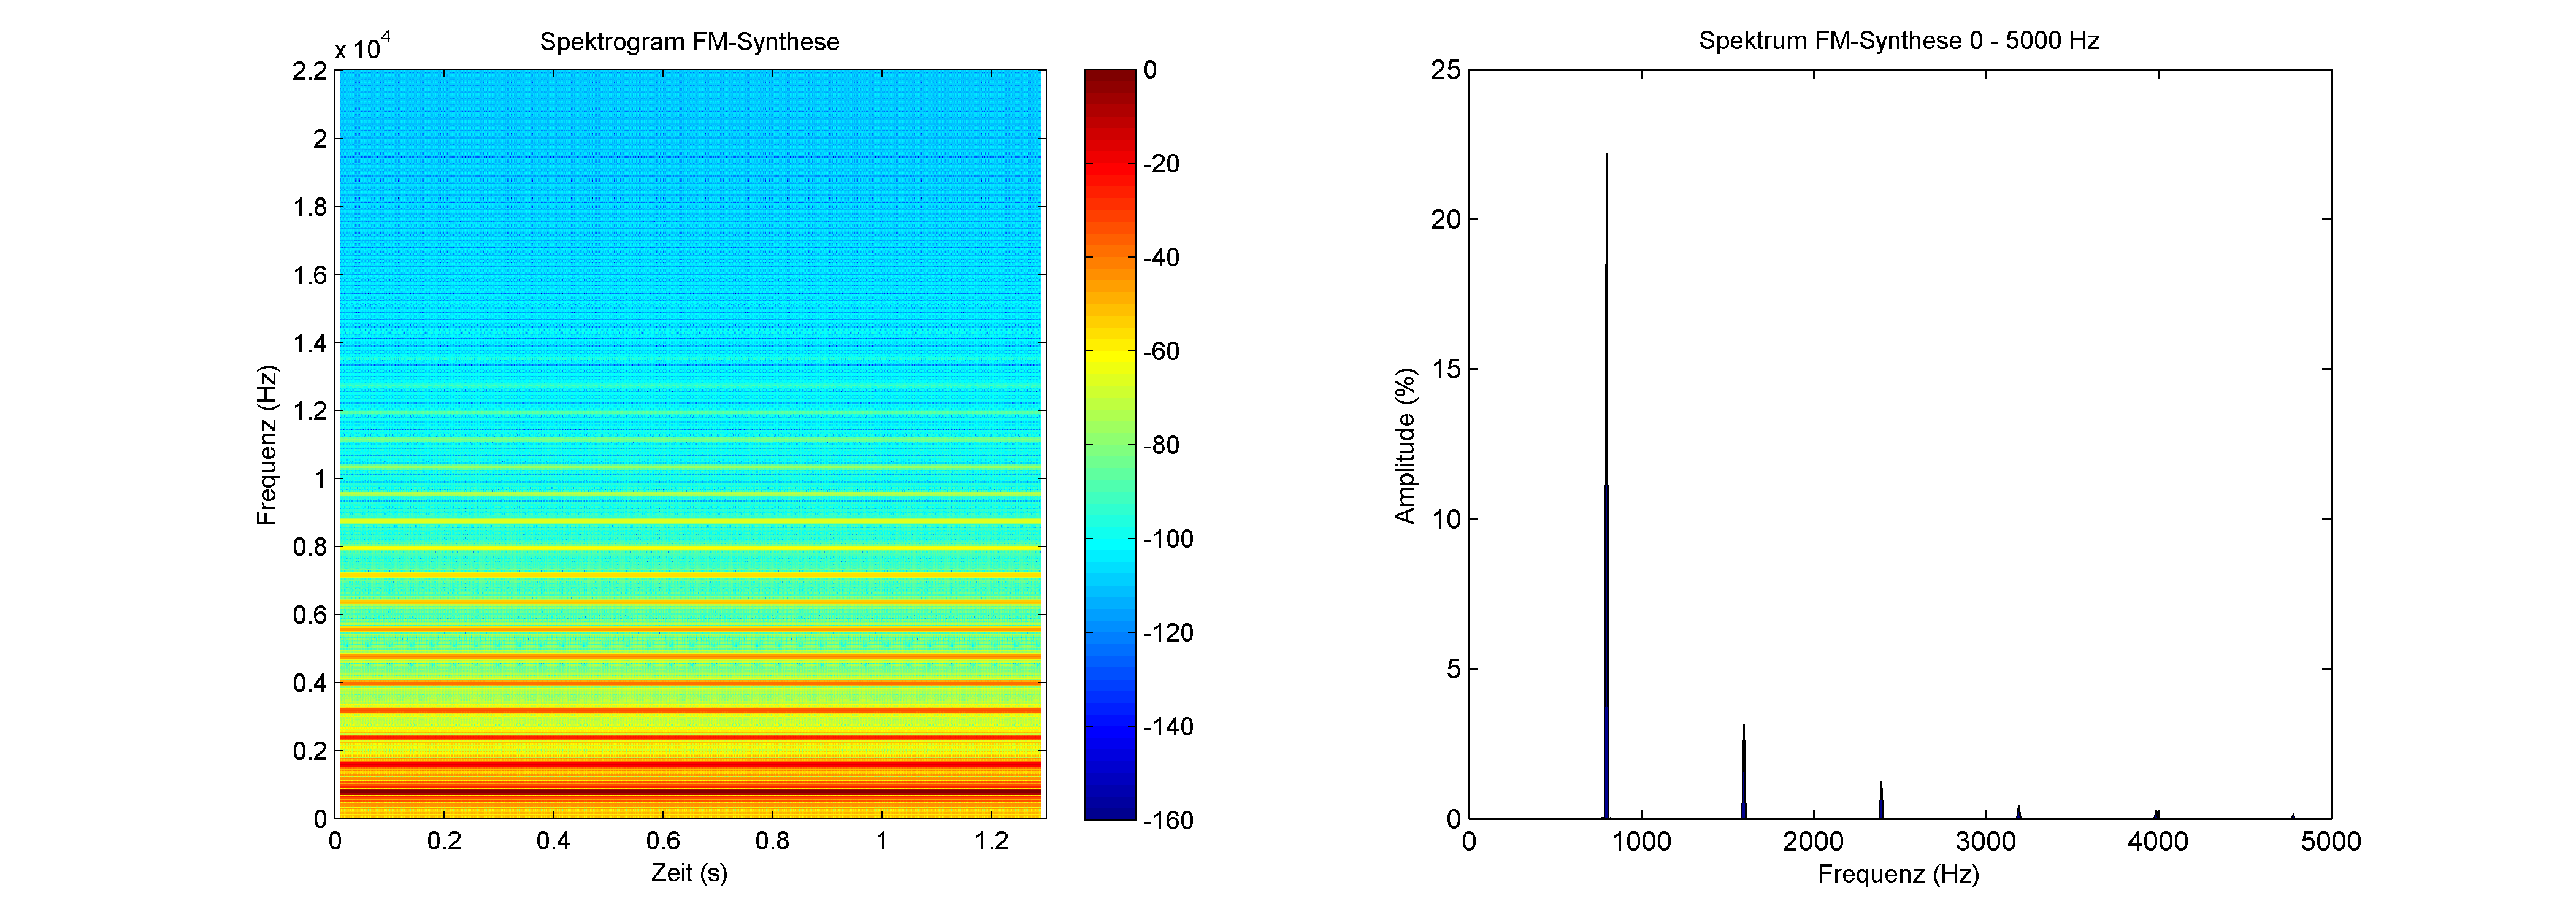
\includegraphics[width=1\textwidth]{plotFMSyntheseKomplex4Mod.png}
\caption{Plot des Spektrogramms und des Spektrums der FM-Synthese mit 4 Modulatoren und den Parametern $f_c = 791 Hz$, $f_{m1} = f_{m2} = f_{m3} = f_{m4} = f_c$, $I_1 = 0.3$, $I_2 = 0.5$, $I_3 = 1$ und $I_4 = 1$}
\label{fig:plotFMSyntheseKomplex4Mod}
\end{figure}

Da die FM-Synthese mit den in Abbildung \ref{fig:plotFMSyntheseKomplex4Mod} genannten Parametern ein zufriedenstellendes Signal erzeugt, kann jetzt mit der Veredlung des Tones begonnen werden. Zuerst wird dem Signal ein Vibrato hinzugefügt. Durch das Hinzufügen des Vibratos, schwingt der erzeugte Ton leicht und wirkt lebendiger und nicht so künstlich. Dies kann bewerkstelligt werden indem die Modulationsfrequenz leicht erhöht oder verringert wird. Auch hierbei muss experimentiert werden, welche Erhöhung der Modulationsfrequenz das gewünschte Ergebnis erzeugt. Als sehr ähnlich zum Originalton hat sich in diesem Fall eine Erhöhung um 2.5 Hz herausgestellt. Unsere neue Modulationsfrequenz ist somit $f_m = f_c + 2.5$. In Abbildung \ref{fig:spektrumFMSyntheseVibrato} wird die Auswirkung des Vibratos sichtbar, es bilden sich um die Seitenfrequenzen weitere recht gering ausgeprägte Frequenzausschläge.

\begin{figure} [ht]
\centering
  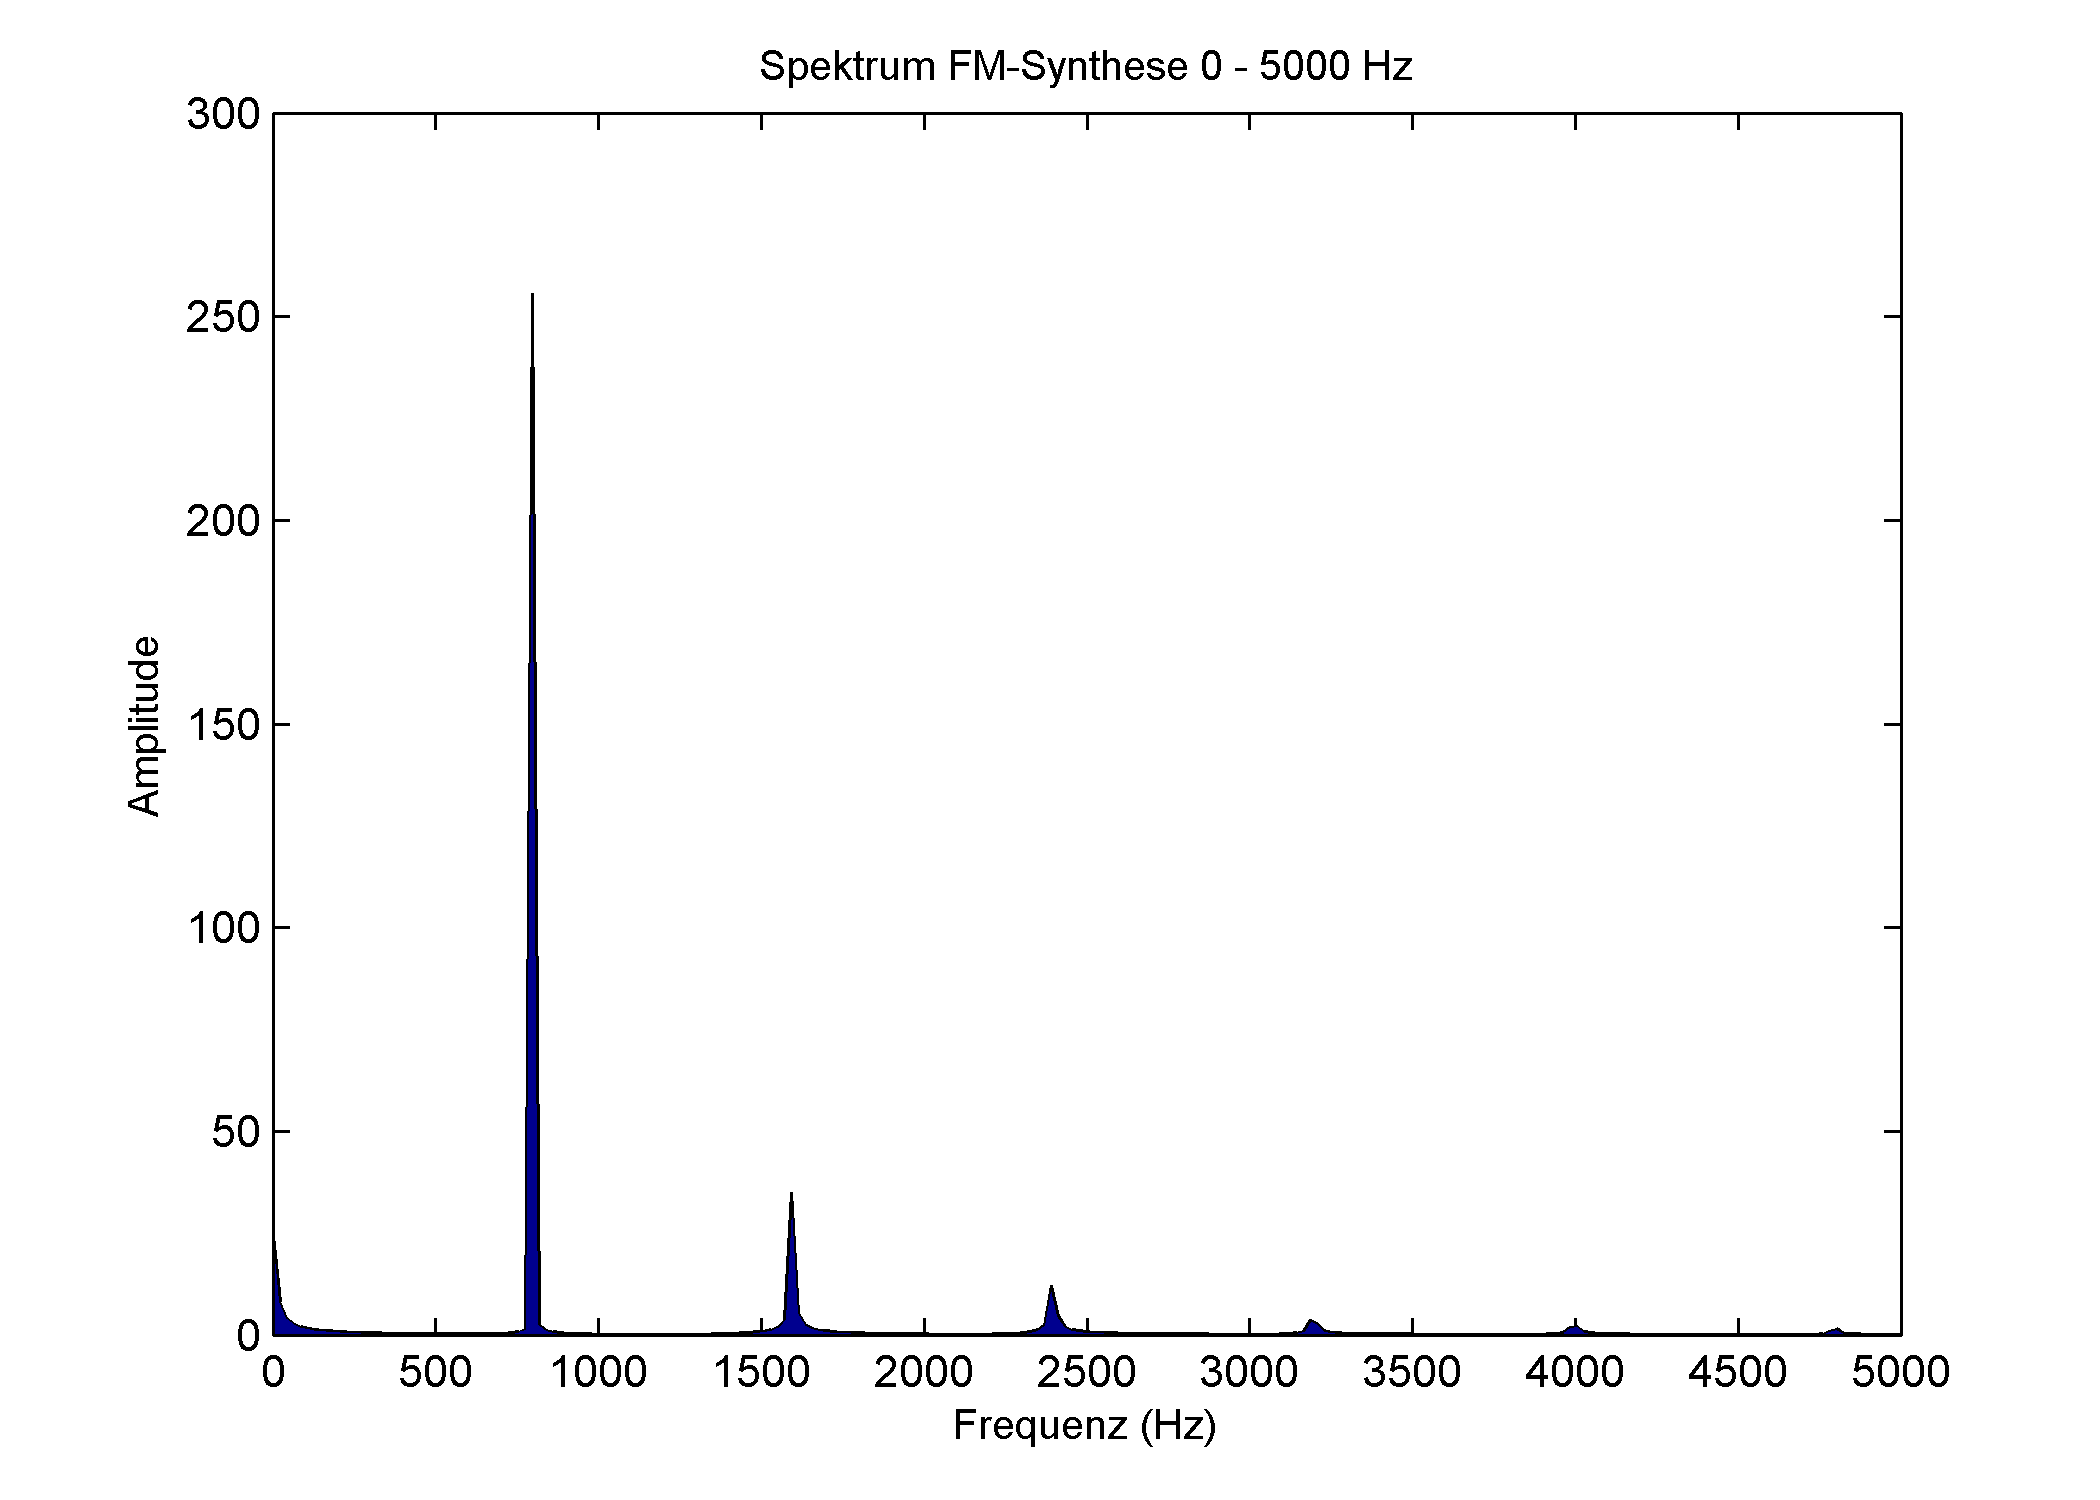
\includegraphics[width=0.5\textwidth]{spektrumFMSyntheseVibrato.png}
\caption{Plot des Spektrums der FM-Synthese mit 4 Modulatoren, Vibrato und den Parameter $f_c = 791 Hz$, $f_{m1} = f_{m2} = f_{m3} = f_{m4} = f_c + 2.5$, $I_1 = 0.3$, $I_2 = 0.5$, $I_3 = 1$ und $I_4 = 1$}
\label{fig:spektrumFMSyntheseVibrato}
\end{figure}

Der nächste wichtige und einfach hinzuzufügende Bestandteil des synthetisierten Tones ist die ADSR-Hüllkurve. Um generell eine Querflöte nachzuahmen wäre eine Hüllkurve wie in Abbildung \ref{fig:adsrFlute} (links) gezeigt möglich. Allerdings wird versucht das Klangbild des Tones der Querflöte so gut wie möglich nachzuahmen, hierfür wurde eine komplexere Hüllkurve nach dem Beispiel der Waveform des originalen Tones generiert. Bei dieser Hüllkurve wurde Attack, Decay und Release von der allgemeinen Hüllkurve übernommen und die Sustain Phase angepasst, zu sehen in Abbildung \ref{fig:adsrFlute} (rechts). 

\begin{figure} [ht]
\centering
  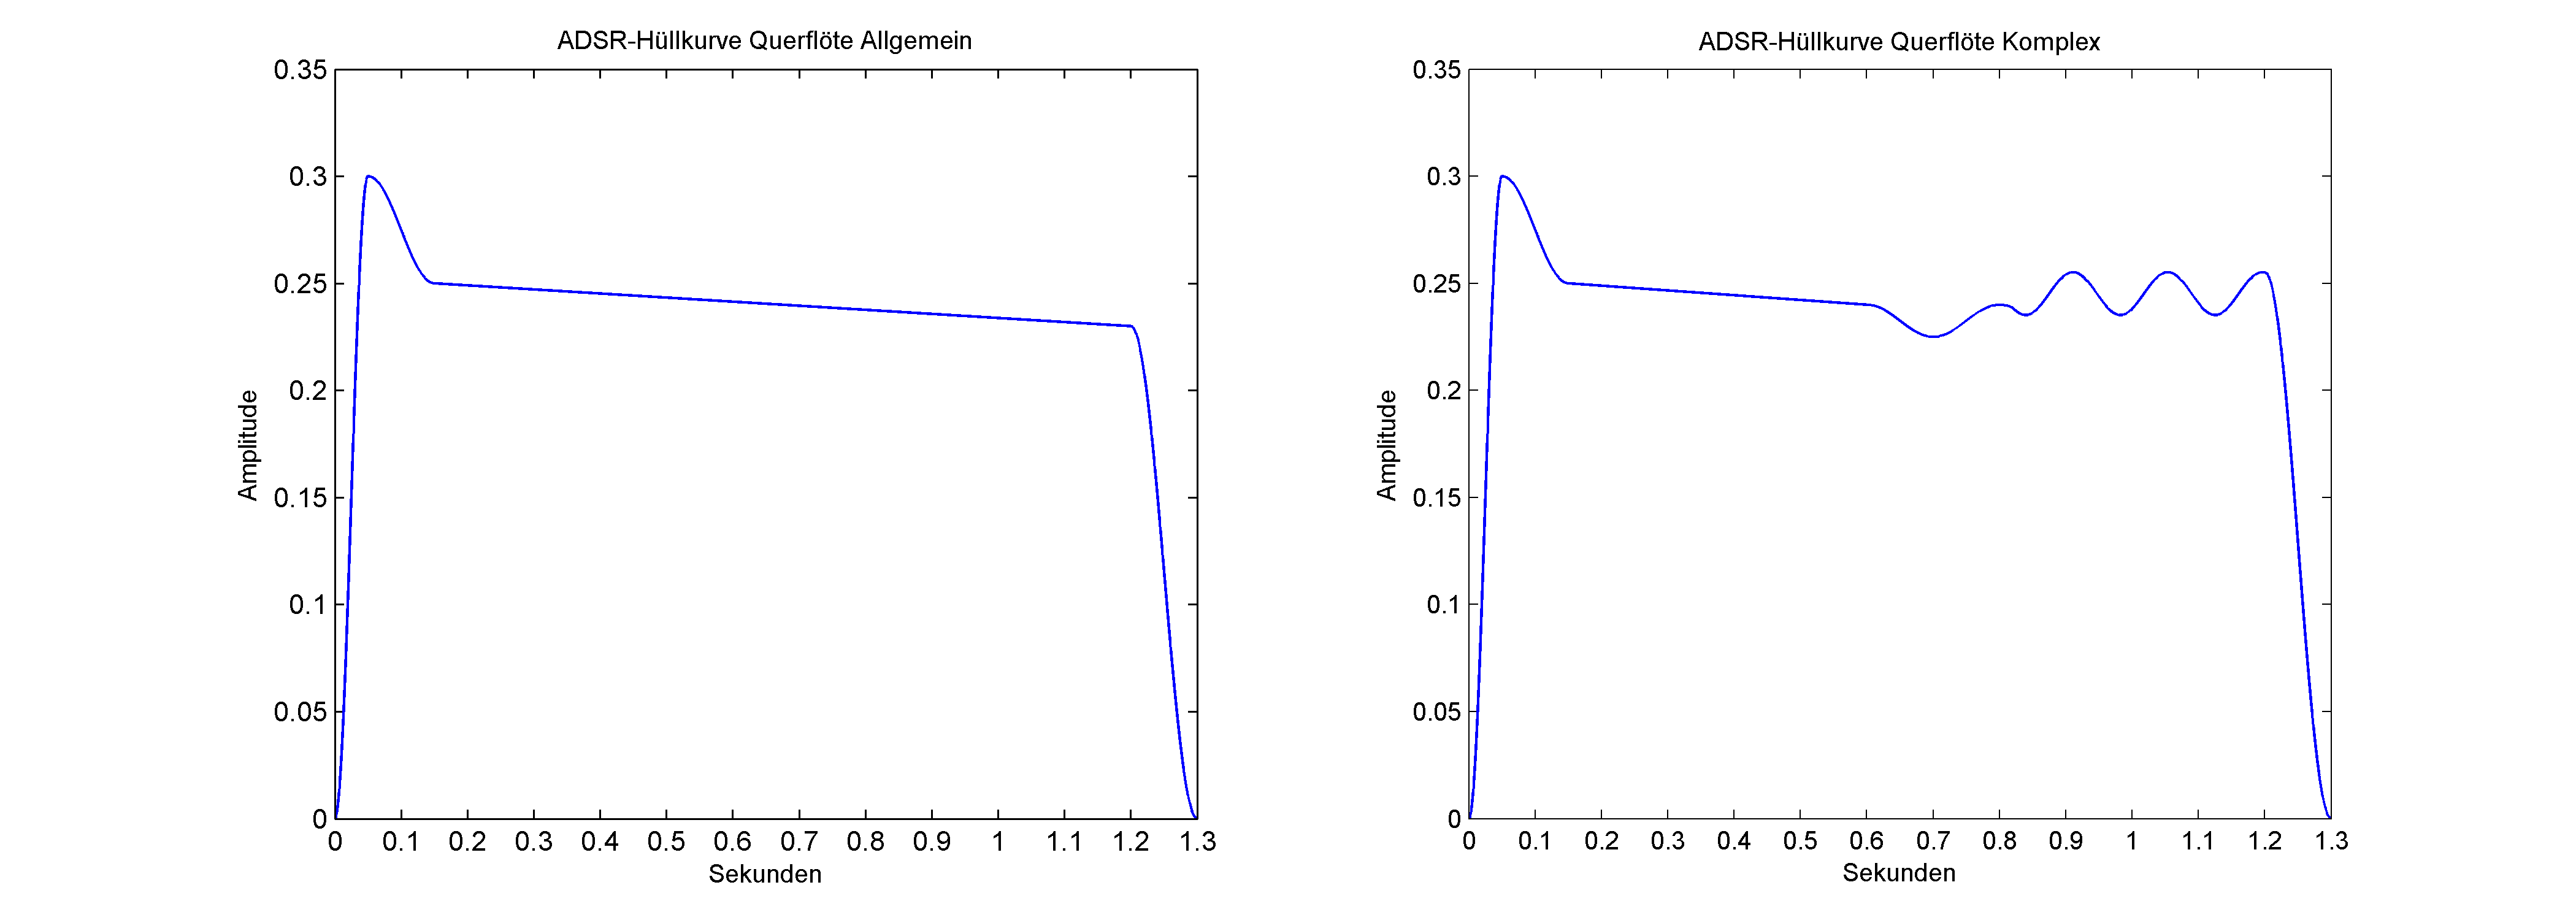
\includegraphics[width=1\textwidth]{adsrFlute.png}
\caption{Plot der ADSR-Hüllkurve einer Querflöte und der hier genutzten, komplexeren Hüllkurve}
\label{fig:adsrFlute}
\end{figure}

Nach Hinzufügen der ADSR-Hüllkurve, fällt im Spektrogramm auf, dass die Seitenfrequenzen trotz geringerer Amplitude bei Attack und Release Phase einen größeren Ausschlag als beim Instrument aufweisen. Dieser Ausschlag kann verringert werden, indem der Modulationsindex mit der ADSR-Hüllkurve variiert wird. Durch diese Anpassung steigt die Anzahl der Seitenfrequenzen zu Beginn des Klangs an und setzten somit verzögert ein. Beim Abklingen werden die Seitenfrequenzen ebenfalls abgeschwächt und ähneln dem Original etwas mehr.

Nachdem Vibrato, variabler Modulationsindex und ADSR-Hüllkurve hinzugefügt wurden, hat sich das Spektrogramm zur Abbildung \ref{fig:plotFMSyntheseKomplex4Mod} kaum geändert. Es wird nur der Vibrato durch die etwas breiteren Seitenfrequenzen und die ADSR-Hüllkurve durch Ansteigen des Spektrums zu Beginn des Tones und Abfallen des Spektrums nach 1.2 Sekunden sichtbar. Der Ton ähnelt in Tonhöhe und Intensität dem originalen Querflötenton schon stark. Allerdings fehlen noch die typischen Blas- und Luftverwirbelungsgeräusche sowie das sehr dominante Anblasgeräusch. Um die typischen Blasgeräusche zu erzeugen wird zunächst ein Rauschen mittels Feedback-FM-Synthese mit hohem Modulationsindex erzeugt. Würde das Rauschen ohne weitere Arbeitsschritte dem synthetisierten Signal hinzugefügt, könnte es stark herausgehört werden. Um dies zu verhindern muss das Rauschen vorerst gefiltert werden. Hierzu wird ein Multibandpassfilter erstellt. In Abbildung \ref{fig:multiBandPassFilter} ist der genutzte Filter grafisch dargestellt. Wie am Bild ersichtlich, ist der Filter durchaus komplex. Ein besonders großer Ausschlag ist am Anfang des Frequenzspektrums zu sehen. Dieser befindet sich zwischen 800 und 1600 Hz. Gerade dieses Frequenzband ist bei der originalen Querflöte stark mit Rauschen ausgeprägt. Zusätzlich wurden Frequenzbänder zwischen 1.600 und 10.000 Hz, mit fallender Amplitude, angelegt. Zwischen 11.000 Hz und 12.000 Hz ist ein weiteres Frequenzband mit starker Ausprägung modeliert, da bei diesen Frequenzen besonders die Blas- und Luftverwirbelungsgeräusche auftreten. Oberhalb der 12.000 Hz wurden noch weitere Frequenzbänder mit niedrigerer Amplitude erstellt. Diese sollen ein Grundrauschen abbilden.

\begin{figure} [h!t!b!]
\centering
  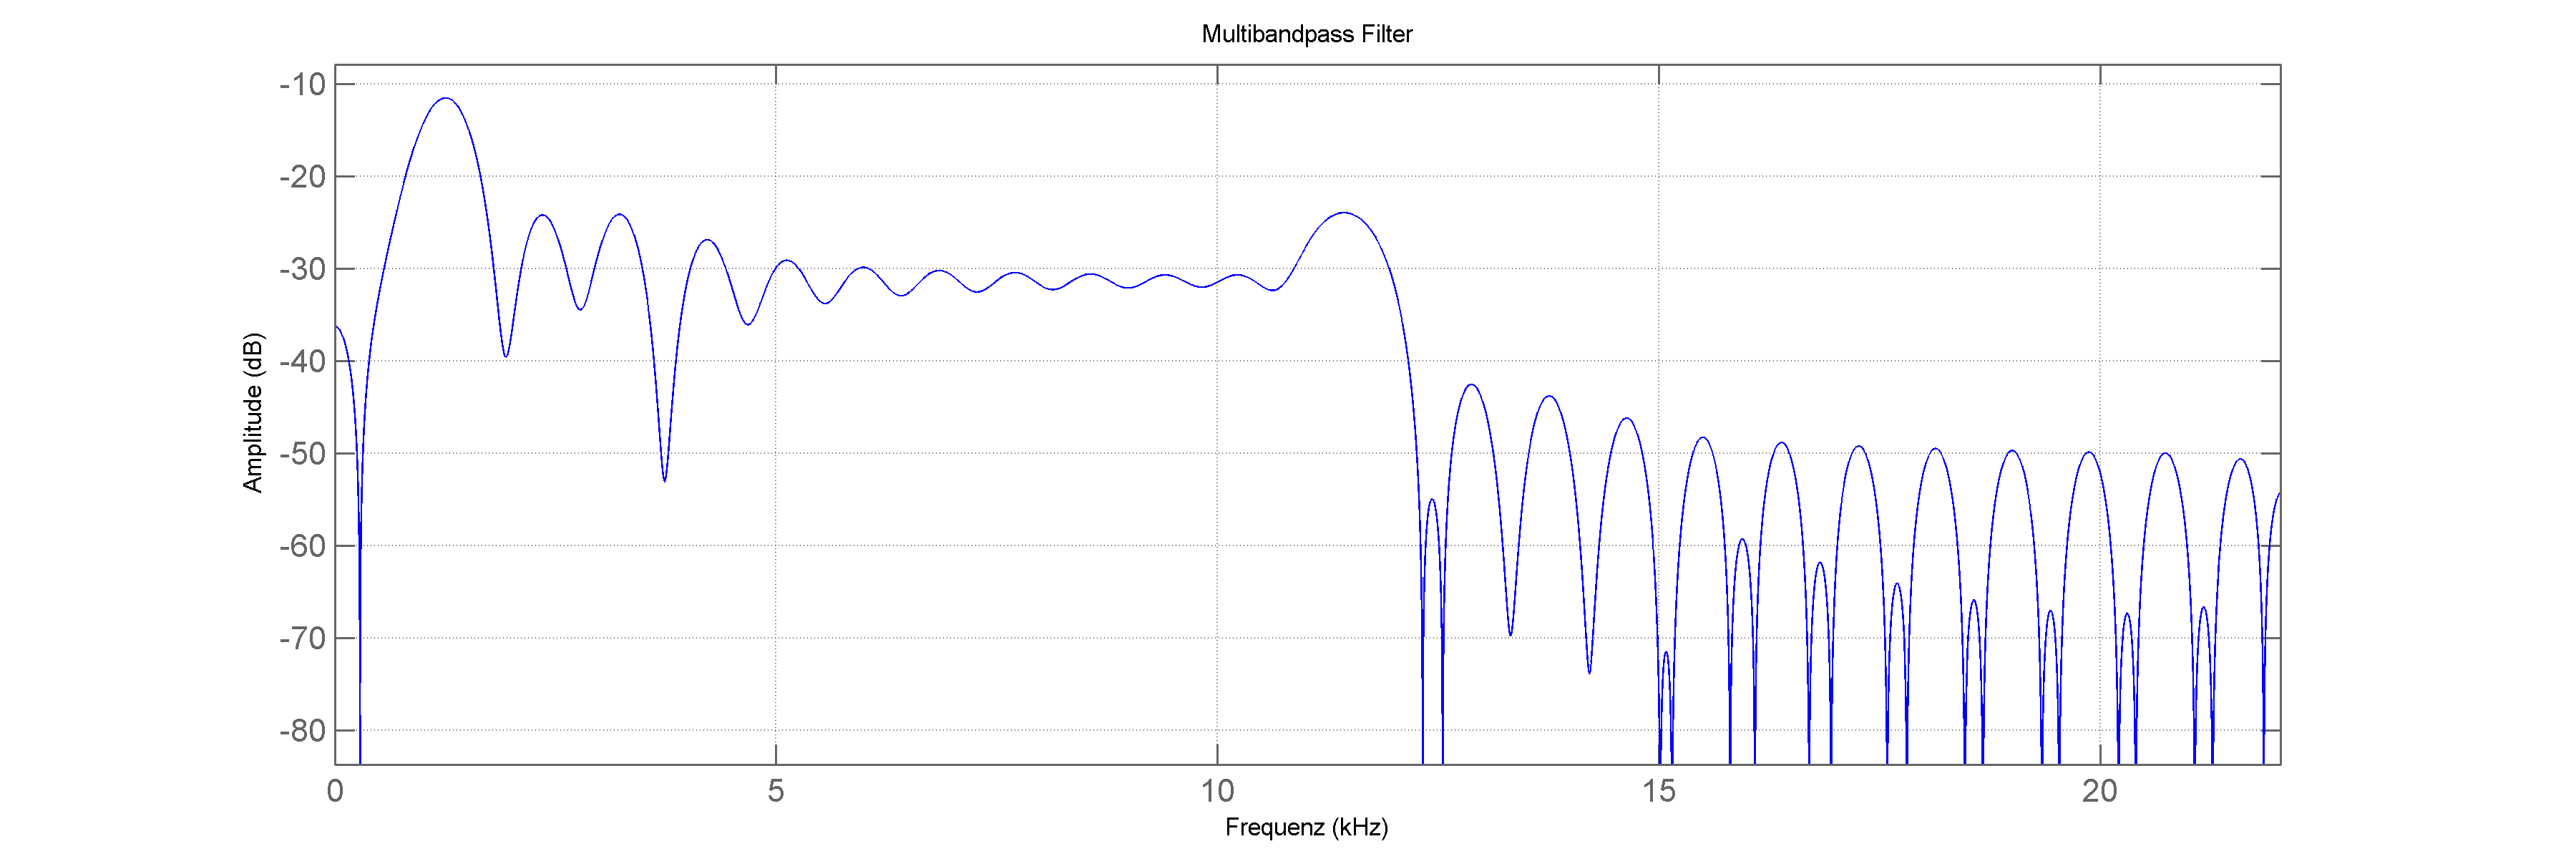
\includegraphics[width=1\textwidth]{multiBandPassFilter.png}
\caption{Plot des Multibandpassfilters der zum Filtern des mit Feedback-FM-Synthese erzeugten Rauschens genutzt wurde}
\label{fig:multiBandPassFilter}
\end{figure}

Das gefilterte Rauschen wird anschließend noch mit einer ADSR-Hüllkurve veredelt. Dieser Schritt ist nötig, da während der Attack Phase des original Tones, wie im Spektrogramm in Abbildung \ref{fig:plotFluteOrig} zu sehen, das Rauschen durch das Anblasen des Instrumentes sehr scharf heraus sticht. Zusätzlich kann noch ein sehr leises Rauschen der Feedback-FM-Synthese ohne Filter über das ganze Frequenzspektrum gelegt werden, um auch in den höheren Frequenzen einen leichten Ausschlag im Spektrogramm kenntlich zu machen. 

Trotz des verstärkten Rauschens zu Beginn des Tones, fehlt noch das stark hörbare Anblasgeräusch. Beim Betrachten des Spektrums und des Spektrogramms fallen noch zwei recht starke Ausschläge zu Beginn des Signals auf. Ein Ausschlag befindet sich bei 904 Hz und der Zweite bei 1182 Hz. Beide Frequenzen können mit einem einfachen Sinus erzeugt und mit einer ADSR-Hüllkurve, die nur eine kurze Attack Phase aufweist und danach komplett abfällt, modelliert und zum Signal hinzugefügt werden. In Abbildung \ref{fig:plotFMSyntheseComplete} ist das Ergebnis der FM-Synthese mit den in diesem Kapitel besprochenen Veredelungen gezeigt. In den Plots sind die Ähnlichkeiten zum originalen Ton deutlich sichtbar.

\begin{figure} [h!t!b!]
\centering
  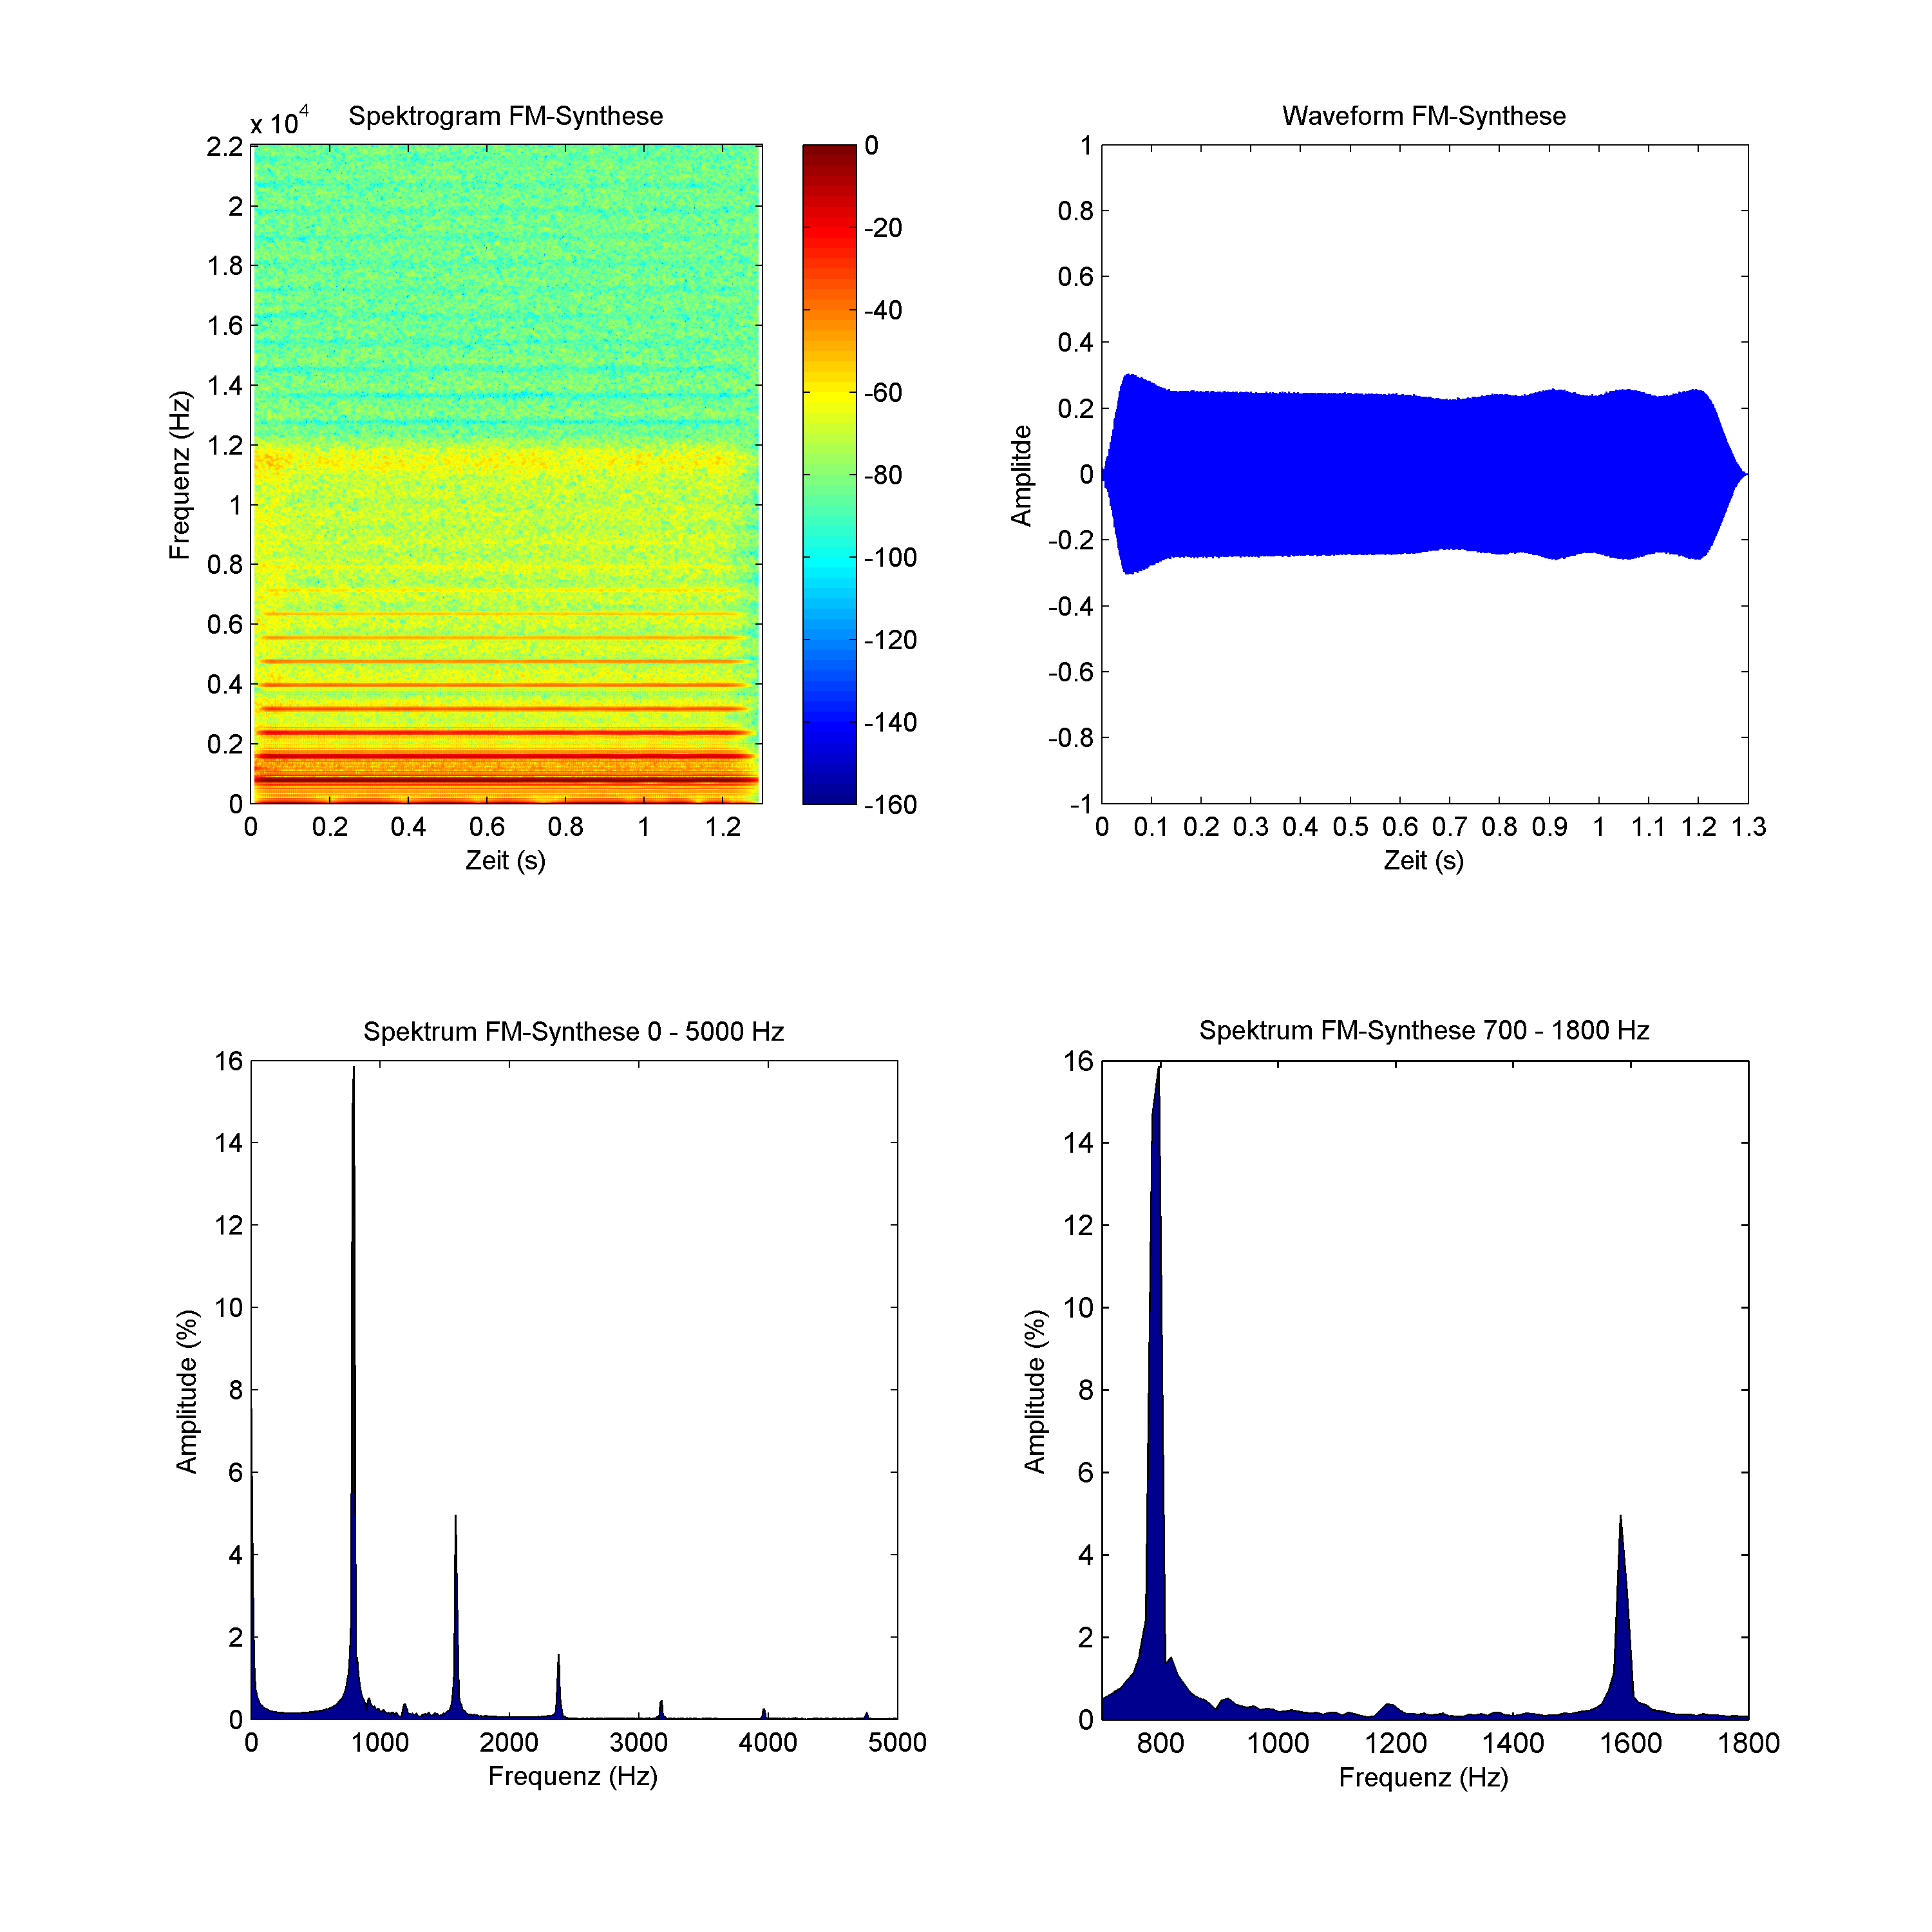
\includegraphics[width=1\textwidth]{plotFMSyntheseComplete.png}
\caption{Plot des fertigen Tones der FM-Synthese mit 4 Modulatoren, ADSR-Hüllkurve, Variablem Modulationsindex, Vibrato, Rauschen, Variabler Trägerfrequenz und Anblasgeräusch}
\label{fig:plotFMSyntheseComplete}
\end{figure}

Der in diesem Kapitel synthetisierte Ton nähert sich dem originalen Flötenton stark an. Sowohl die Tonhöhe wie auch das Klangbild konnten sehr gut nachgebildet werden. Durch das genutzte Vibrato, dem variablem Modulationsindex und der variablen Trägerfrequenz wirkt der erzeugte Klang lebendig. Einzig das scharfe Anblasgeräusch unterscheidet sich noch etwas von dem des originalen Tones. Wäre man allerdings nicht in der Lage die beiden Töne zu vergleichen könnte der synthetisierte Ton durchaus als ein echtes Instrument erkannt werden. Dieses Ergebnis zeigt, dass es sehr wohl möglich ist, mit der FM-Synthese einen natürlich wirkenden Instrumententon zu erzeugen. Allerdings ist dies mit erheblichem Aufwand verbunden.


\FloatBarrier
\subsection{Implementierung eines FM-Synthesizers zur Demonstration der Synthese Parameter}

Zu Beginn dieser Arbeit wurde zum besseren Verständnis der FM-Synthese ein kleiner Software Synthesizer in C++ mit der Hilfe des JUCE Frameworks implementiert. Das JUCE Framework wurde hierfür ausgewählt, da es gerade für ein Audioprogramm gut geeignet ist. Es bietet bereits Funktionen zur Ausgabe eines Audio Signals und Möglichkeiten zur Erstellung einer Benutzeroberfläche. Zudem ist es Cross Plattform fähig.

Zunächst wurde eine einfache FM-Synthesizer Klasse geschrieben und diese an das Audio Ausgabesystem des JUCE Frameworks angebunden. Dabei ruft die Soundkarte eine Methode des Programms auf und erwartet, dass der übergebene Puffer mit Audiodaten gefüllt wird. Das Programm füllt den gegebenen Puffer mit Daten die mit der FM-Synthesizer Klasse generiert wurden. Später wurde das Programm dann noch um die visuelle Darstellung des erzeugten Audiosignals erweitert. Außerdem ist es möglich dem FM-Synthesizer einen Hüllkurvengenerator zu übergeben, welcher bei der Erzeugung des Audiosignals den Amplitudenwert für die einzelnen Samples bereitstellt. Die Amplitudenwerte werden ebenfalls visuell dargestellt.

Da gerade die Änderung der Parameter und das jeweils resultierende Klangbild zum Verständnis hilfreich sind, wurden Möglichkeiten in das Programm eingebaut um sowohl den Modulationsindex als auch die Modulationsfrequenz sowie die Oktave zu ändern. Das Ändern der Parameter ist mittels einfachem Tastendruck möglich. Zusätzlich wurde das Programm so angepasst, dass es mittels Tastendruck ermöglicht wird verschiedene Töne zu spielen. Die Tasten "'C"', "'D"', "'E"', "'F"', "'G"', "'A"' und "'B"' entsprechen dabei jeweils ihrem tonalem Äquivalent. Beim Drücken der Taste startet die Hüllkurve in die Attack Phase, geht dann über in die Decay und schließlich in die Sustain Phase. Wird die Taste losgelassen startet die Release Phase und der Ton klingt ab. Mit den Tasten "'1"' und "'2"' kann der Modulationsindex inkrementiert sowie dekrementiert werden. Um die Modulationsfrequenz zu ändern können die Pfeil hoch und Pfeil runter Tasten genutzt werden. Die Octave lässt sich mit den Tasten "'+"' und "'-"' verändern.

Das entstandene Programm bietet eine gute Möglichkeit die Parameter der FM-Synthese während der Wiedergabe eines Tones zu verändern und hilft so zu verstehen was beim Ändern dieser passiert. Natürlich ist das entstandene Programm nicht so flexibel und mächtig wie beispielsweise das Programm FM8 von Native Instruments. Trotzdem bietet es einen einfachen Einstieg in die FM-Synthese und der für Parameter resultierenden Spektren und Klänge. Somit wurde das Ziel, das mit der Programmierung des Tools gesetzt wurde, erreicht.
\FloatBarrier
